\documentclass[11pt,a4paper]{article}
\usepackage[margin=2cm]{geometry}
\usepackage[T1]{fontenc}
\usepackage{lmodern,microtype,graphicx,booktabs,enumitem,xcolor,hyperref,titlesec,amsmath,float}
\usepackage[most]{tcolorbox}
\definecolor{navy}{HTML}{1D2F82}\definecolor{warn}{HTML}{C0392B}\definecolor{ok}{HTML}{2E8B57}
\hypersetup{colorlinks,linkcolor=navy,urlcolor=navy}
\titleformat{\section}{\Large\bfseries\color{navy}}{\thesection}{0.6em}{}
\titleformat{\subsection}{\large\bfseries\color{navy}}{\thesubsection}{0.5em}{}
\setlist{itemsep=2pt,topsep=3pt}
\graphicspath{{../figures/}{../diagrams/}}
\newtcolorbox{say}{colback=navy!4,colframe=navy,boxrule=0.6pt,arc=2pt,left=6pt,right=6pt,top=3pt,bottom=3pt,fonttitle=\bfseries,title=Say this}
\newtcolorbox{careful}{colback=warn!4,colframe=warn,boxrule=0.6pt,arc=2pt,left=6pt,right=6pt,top=3pt,bottom=3pt,fonttitle=\bfseries,title=Be careful}
\newtcolorbox{owned}{colback=orange!6,colframe=orange!80!black,boxrule=0.6pt,arc=2pt,left=6pt,right=6pt,top=3pt,bottom=3pt,fonttitle=\bfseries,title=Corrections (own these)}
\newtcolorbox{readfig}{colback=ok!5,colframe=ok,boxrule=0.6pt,arc=2pt,left=6pt,right=6pt,top=3pt,bottom=3pt,fonttitle=\bfseries,title=How to read this figure}
\newcommand{\figread}[4]{\begin{readfig}\textbf{Axes:} #1\par\textbf{Good vs bad:} #2\par\textbf{Key number:} #3\par\textbf{Takeaway:} #4\end{readfig}}
\newcommand{\qa}[2]{\par\smallskip\noindent\textbf{Q: #1}\par\noindent\hspace*{1em}\begin{minipage}[t]{\dimexpr\linewidth-1em}#2\end{minipage}\par}
\newcommand{\degC}{\textdegree C}

\title{\color{navy}\textbf{Final Review Reading Guide}\\[4pt]\large Design of a Temperature-Compensated PLL Frequency Synthesiser}
\author{For Viju Sanjai --- Final Review (Review III), 28.10.2026\\ Team: Aaryan Dogra, Yugeshwaran, Viju Sanjai; Guide: Dr.\ B.\ Bindu}
\date{}
\begin{document}
\maketitle
\vspace{-1.5em}
\noindent This is a reading document. It explains what was done, how to read every result plot, what each number means, and how to answer an examiner. All numbers come from the generated results files in the repository (\texttt{results/final\_numbers.md}, \texttt{results/corner\_audit/FINDINGS.md}, \texttt{results/comp/mc\_v2\_analysis.txt}, \texttt{results/loop/campaign/summary.csv}). Several Review~2 claims were corrected after Review~2; those old claims appear \emph{only} in Section~\ref{sec:corr}. If an examiner quotes an old number from the Review~2 slides, check that section first.

\tableofcontents
\newpage

%=====================================================================
\section{The story in 60 seconds}
\begin{say}
A ring-oscillator VCO changes frequency with temperature, so a PLL built around it has to work harder as the chip heats up. We built a complete integer-N charge-pump PLL in the open sky130B process and simulated it in ngspice. The VCO drifts 8.5\% over $-40$ to 85\,\degC\ at the typical corner, and between 1.5\% and 17.5\% across 11 process corners. We add a correction voltage $k_1(T-27)+k_2(T-27)^2$ to the VCO control voltage. Fitted properly on the measured frequency surface and verified at held-out temperatures, the 2nd-order version cuts the typical-corner span from 8.51\% to 0.20\% and meets our $\pm0.3\%$ target at 8 of 11 corners; the other three are 0.30, 0.33 and 0.36\%, just outside. With transistor mismatch (72 virtual chips) the correction removes about 17 MHz of the 20 MHz drift, leaving about 3 MHz (1.2--1.4\%): a mismatch floor that one global correction cannot remove. Here 2nd order is not statistically better than 1st order, which is an honest and correct finding. The closed loop (retuned to $\zeta\approx0.70$) locks to $8\times f_{ref}$ = 226.17 MHz at all 11 corners from both a coarse and a true 0 V start, inside the 2\,$\mu$s spec, with one honest exception: ss at 85\,\degC\ takes 2083 ns, 4\% over.
\end{say}

\noindent\textbf{What the final review adds over Review 2}
\begin{enumerate}
\item \textbf{Corner audit:} we were asked why sf/fs numbers look out of range; we investigated and found the PDK's skew corners are simply wider than ss/ff. We added a textbook $3\times3$ corner set and report 11 corners.
\item \textbf{Corrected compensation:} the earlier coefficients were limited by a wrong $K_{VCO}$; the new fit meets spec at tt and 8/11 corners.
\item \textbf{Corrected Monte Carlo:} $n=72$ with the corrected coefficients.
\item \textbf{Full closed-loop campaign:} 28 transistor-level runs across 11 corners and temperatures.
\end{enumerate}

%=====================================================================
\section{The system and each block}
\begin{center}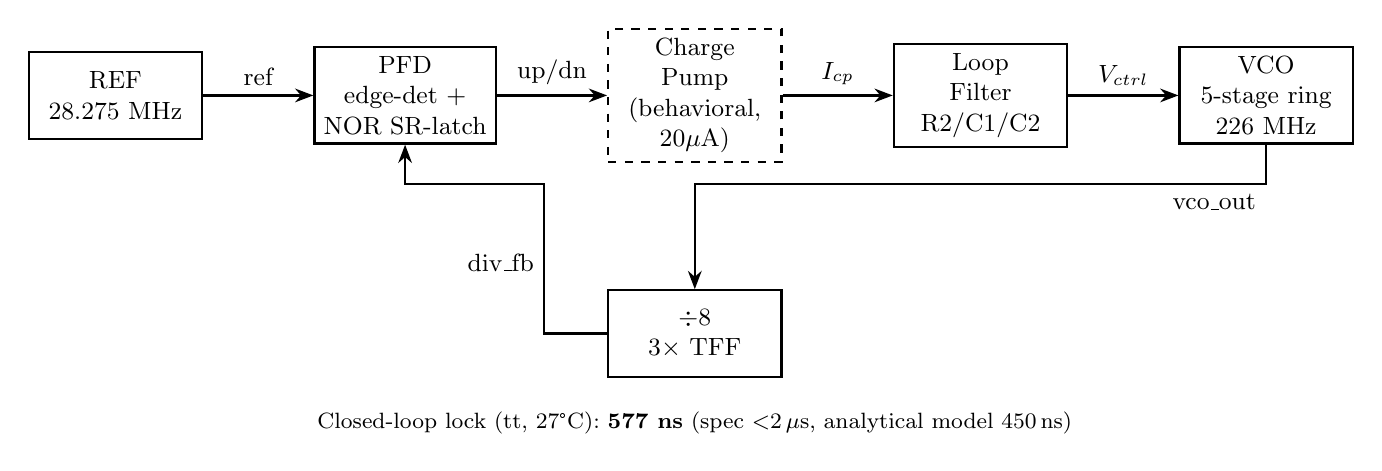
\includegraphics[width=\linewidth]{pll_block_diagram.png}\end{center}
\begin{itemize}
\item \textbf{Reference:} 28.275 MHz. Output is $8\times$, 226.2 MHz, at $V_{ctrl}=0.9$ V, tt, 27\,\degC.
\item \textbf{PFD (phase-frequency detector):} compares reference and divided-VCO edges and produces UP/DN pulses proportional to the phase error. Built from edge detectors and NOR SR-latches (resettable D flip-flops failed because the asynchronous reset fought the latch feedback in our hand-built cells).
\item \textbf{Charge pump:} UP/DN pulses become $\pm20\,\mu$A current pulses into the loop filter. It is a \emph{behavioural} (ideal) model, not transistors. It runs at $5\times$ until the first divider edge (cold-start boost).
\item \textbf{Loop filter:} $R_2=3.6$ k$\Omega$ in series with $C_1=68$ pF, with $C_2=6.8$ pF in parallel. It integrates current into $V_{ctrl}$. $R_2$ adds the zero that stabilises the loop; $C_2$ smooths ripple. ($R_2$ was 1.7 k$\Omega$ in Reviews 1--2.)
\item \textbf{VCO:} a 5-stage current-starved ring. $V_{ctrl}$ sets the starving current, which sets the delay per stage and therefore the frequency.
\item \textbf{Divider $\div8$:} three toggle flip-flops, feeding the divided clock back to the PFD.
\end{itemize}
\begin{center}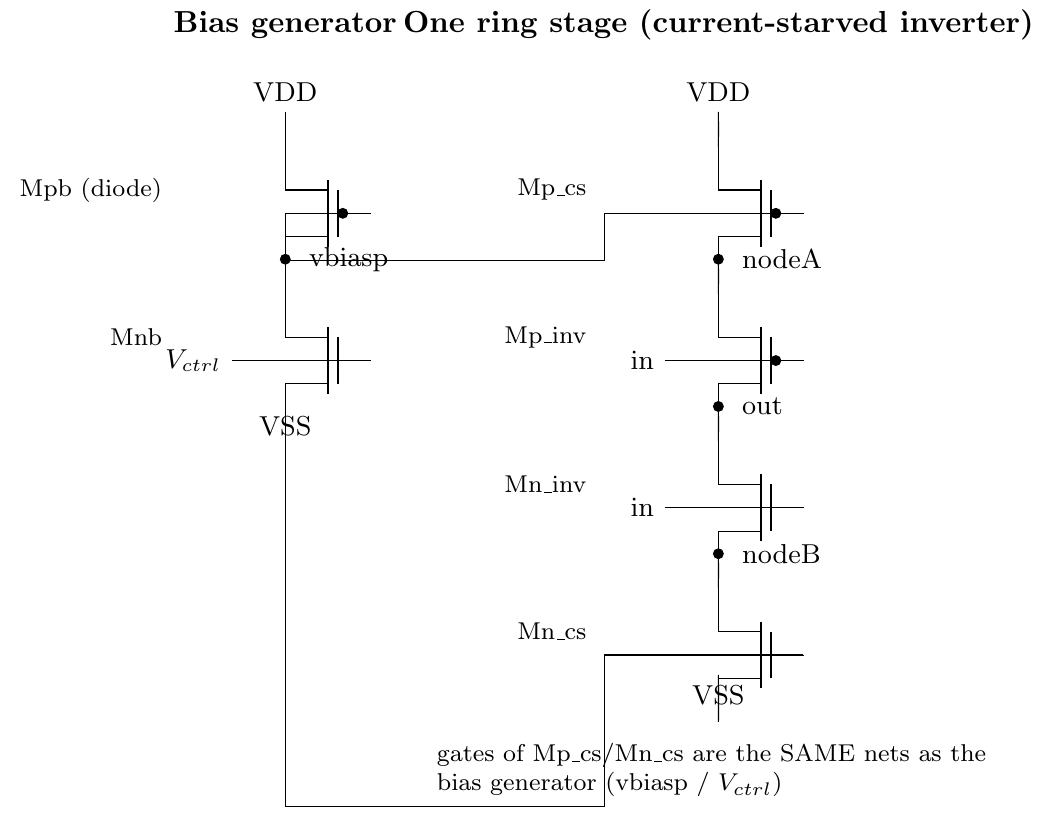
\includegraphics[width=0.46\linewidth]{vco_schematic.png}\hfill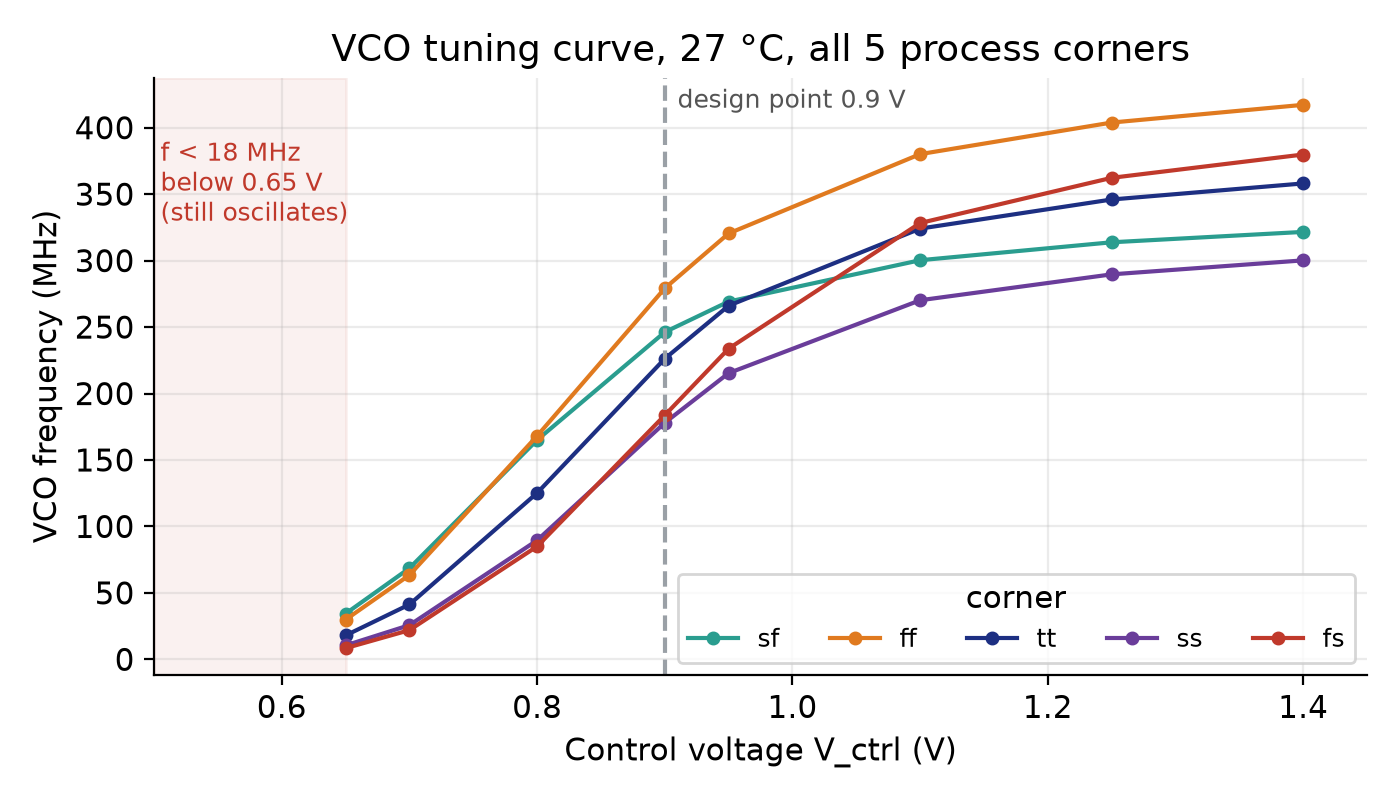
\includegraphics[width=0.52\linewidth]{tuning.png}\end{center}
\figread{x: control voltage $V_{ctrl}$ (V); y: VCO frequency (MHz); one curve per PDK corner at 27\,\degC; dashed line is the 0.9 V design point.}
{A good tuning curve is monotonic and covers the target (226 MHz) well inside its range, which it does. The slope is not constant (S-shape): steep around 0.8--1.0 V, flat above 1.2 V. The curves fan out with process: at 0.9 V ss 178.0 $<$ fs 183.7 $<$ tt 226.2 $<$ sf 246.2 $<$ ff 279.2 MHz.}
{tt tunes 18 MHz at 0.65 V to 358 MHz at 1.40 V; local gain $K_{VCO}\approx890$ MHz/V at 0.9 V (tt).}
{One control voltage covers 226 MHz at every corner, but the voltage needed differs by corner (0.85--0.97 V), which later explains the lock voltages.}

\subsection{$K_{VCO}$ and the low-voltage region}
\noindent $K_{VCO}=df/dV_{ctrl}$ is measured as a central difference at $0.9\pm0.05$ V: tt 887 (about 890) MHz/V; sf/ff/ss/fs: 580/940/820/1020 MHz/V. There is no hard oscillation floor: the ring keeps running in subthreshold (0.63 MHz at 0.5 V, 6.5 MHz at 0.6 V, 18 MHz at 0.65 V). But below about 0.65 V it is under 8\% of the target, so from a 0 V start the divided clock is effectively absent; this is why the cold start needs the boost.

%=====================================================================
\section{Uncompensated drift: the problem we are solving}
\begin{center}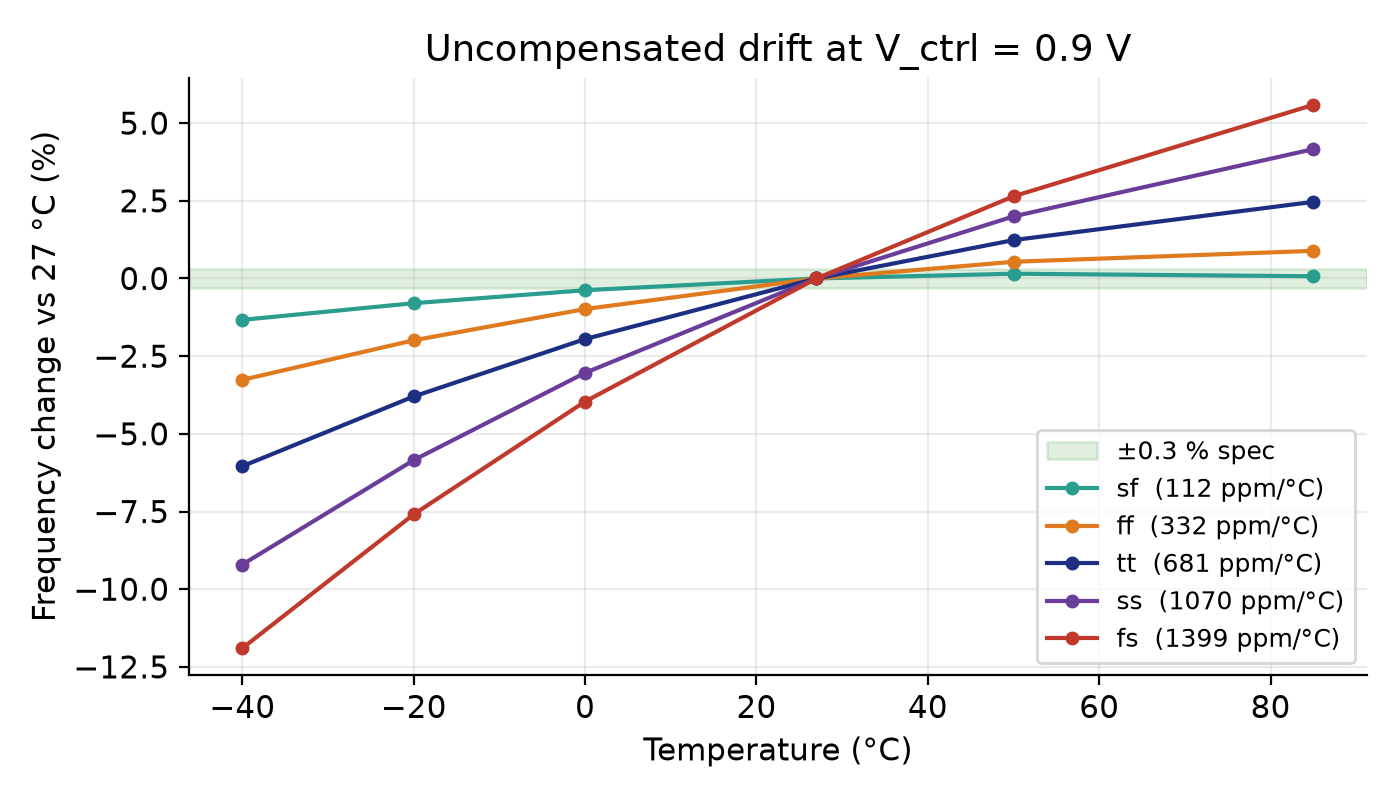
\includegraphics[width=0.62\linewidth]{drift_uncomp.png}\hfill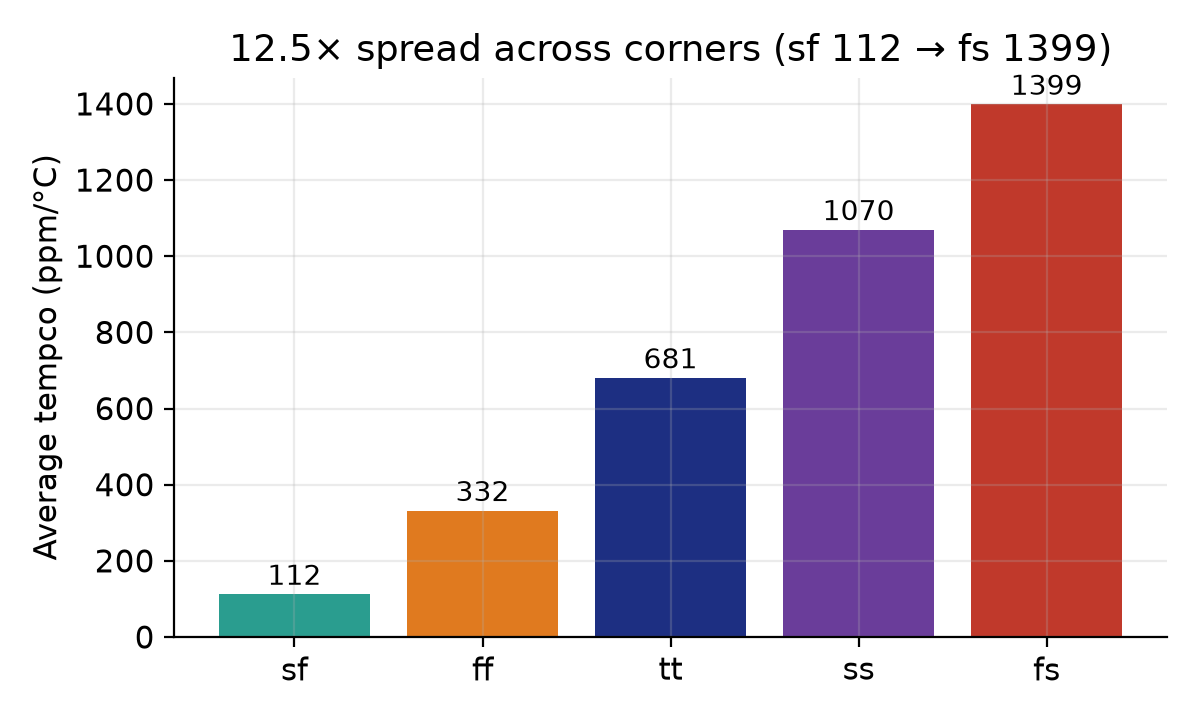
\includegraphics[width=0.36\linewidth]{tempco_bar.png}\end{center}
\figread{left: x temperature (\degC), y frequency change relative to 27\,\degC\ (\%), at fixed $V_{ctrl}=0.9$ V, one line per PDK corner; the green band is our $\pm0.3\%$ spec. Right: bar chart of the average tempco in ppm/\degC.}
{Good would be a flat line inside the green band. Every corner is outside it except that sf only just stays near it. Steeper line = worse.}
{Tempco (PDK corners): sf 112, ff 332, tt 681, ss 1070, fs 1399 ppm/\degC, a 12.5$\times$ spread. Typical-corner span 8.51\%.}
{Frequency \emph{rises} with temperature at this bias, and the amount depends strongly on the process corner, so no single fixed correction suits every chip.}

\noindent Tempco $=(f_{85}-f_{-40})/(f_{27}\cdot125)$. Span is max $-$ min of $f$ over the range, as a \% of $f_{27}$. Procedure: fix $V_{ctrl}=0.9$ V, simulate $T\in\{-40,-20,0,27,50,85\}$\,\degC.

\subsection{Why the drift is curved}
\begin{center}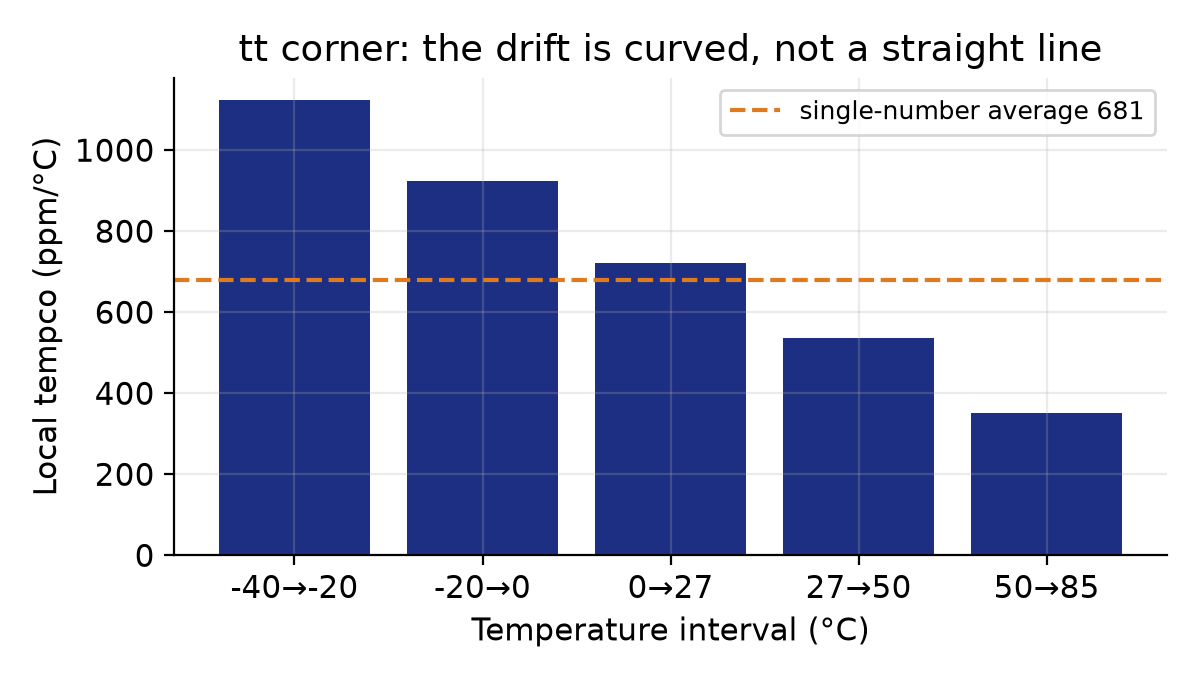
\includegraphics[width=0.55\linewidth]{tt_local.png}\end{center}
\figread{x: temperature interval; y: local tempco (ppm/\degC) over that interval at tt; dashed line is the single-number average.}
{A perfectly linear drift would give equal bars. Ours fall from 1123 (cold) to 352 (hot).}
{Average 681 ppm/\degC, cold end 1123, hot end 352.}
{The drift is curved, so a straight-line (1st-order) correction leaves a bowed residual, which motivates the $(T-27)^2$ term.}

%=====================================================================
\section{Corner audit: why sf/fs numbers looked out of range}
We were asked in review why ff/tt/fs/sf values ``aren't in the ranges they're meant to be''. We audited everything. \textbf{Nothing in the simulations was broken.} What was wrong was how we labelled and expected the corners.

\subsection{Process corners from scratch}
A MOSFET's threshold voltage $V_{th}$, mobility and so drive current vary from die to die and wafer to wafer. A \emph{process corner} is a set of device models with these parameters pushed to an extreme. Two letters: the first for the NMOS, the second for the PMOS. \textbf{t} = typical, \textbf{s} = slow (higher $V_{th}$, lower current), \textbf{f} = fast (lower $V_{th}$, higher current). So \textbf{tt} is typical both, \textbf{ss} both slow, \textbf{ff} both fast, and the \emph{skew} corners \textbf{sf} and \textbf{fs} have one device slow and the other fast. In this PDK, measurement shows \textbf{sf = fast NMOS / slow PMOS} and \textbf{fs = slow NMOS / fast PMOS}. (The PDK only says ``Slow-Fast corner'' without naming devices, and SkyWater's doc tables are inconsistent, so we trust our measurements.) Rule: always say ``fast-NMOS'', never assume ``sf means slow N''.

\subsection{Why NMOS drive sets this VCO}
At $V_{ctrl}=0.9$ V the NMOS starving transistor has an overdrive $V_{gs}-V_{th}$ of only about 0.2 V, since NMOS $V_{th}\approx0.67$ V. The current through it sets the delay. The PMOS starving device is biased through a mirror and is the less limiting device at this bias. So the NMOS corner dominates: at 0.9 V going slow-to-fast NMOS changes $f$ by about 36\%, while slow-to-fast PMOS changes it by only about 10\%. (At $V_{ctrl}=1.4$ V this flips: PMOS 26\% vs NMOS 9\%.)

\subsection{The PDK skew corners are wider than ss/ff}
Extracted threshold shifts versus tt:
\begin{center}\small\begin{tabular}{lrrrr}\toprule
& ss & ff & sf & fs\\\midrule
NMOS $V_{th}$ shift (mV) & +25 & $-25$ & $-36$ & +36\\
PMOS $|V_{th}|$ shift (mV) & +15 & $-23$ & +32 & $-43$\\\bottomrule
\end{tabular}\end{center}
Intuition: we expected skew corners to be milder than ss/ff, lying between them. In this PDK they push each device \emph{further} than ss/ff do. With a small overdrive (0.2 V) an extra 11 mV of $V_{th}$ is about $2\cdot11/230\approx9\%$ of the drive current. So at the VCO bias the skews fall outside the ss--ff envelope.
\begin{center}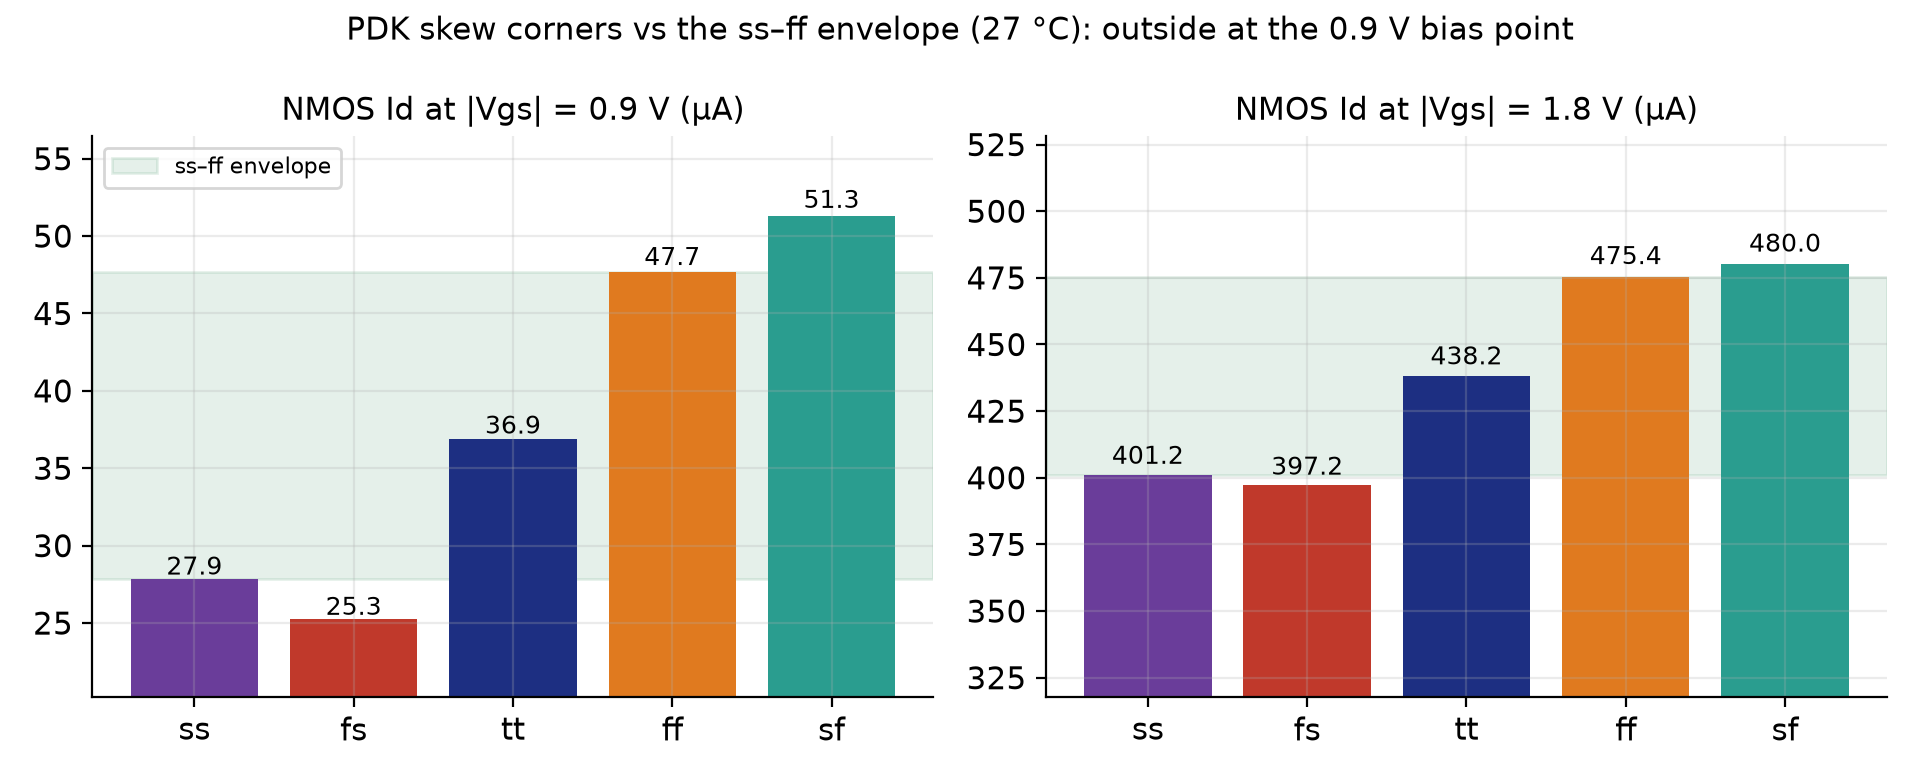
\includegraphics[width=0.85\linewidth]{audit_device_envelope.png}\end{center}
\figread{two bar charts of NMOS drain current of a single 2/0.5\,$\mu$m device at 27\,\degC: left at $|V_{gs}|=0.9$ V ($\mu$A), right at 1.8 V; the green band is the ss--ff range.}
{Textbook behaviour has every bar inside the band. On the left sf (51.3) and fs (25.3) stick out by 8--9\% beyond ff (47.7) and ss (27.9); on the right (strong inversion) all are within 1\%.}
{0.9 V: fs 25.3, ss 27.9, tt 36.9, ff 47.7, sf 51.3 $\mu$A. 1.8 V: ss 401, fs 397, tt 438, ff 475, sf 480 $\mu$A.}
{The skew corners are not weird; at low overdrive the PDK's wider skew definition is amplified. Our VCO happens to sit at low overdrive.}

\subsection{The textbook $3\times3$ corner set}
To give a clean reference we built all nine NMOS $\times$ PMOS combinations (slow/typ/fast each) by swapping the PDK's own NMOS and PMOS model files independently (\texttt{scripts/make\_factorial\_lib.py}). The diagonal reproduces the PDK ss/tt/ff exactly (177.993/226.206/279.178 MHz), a good validity check. Naming: \texttt{nXpY} (X,Y in s/t/f); \texttt{nsps}=ss, \texttt{ntpt}=tt, \texttt{nfpf}=ff.
\begin{center}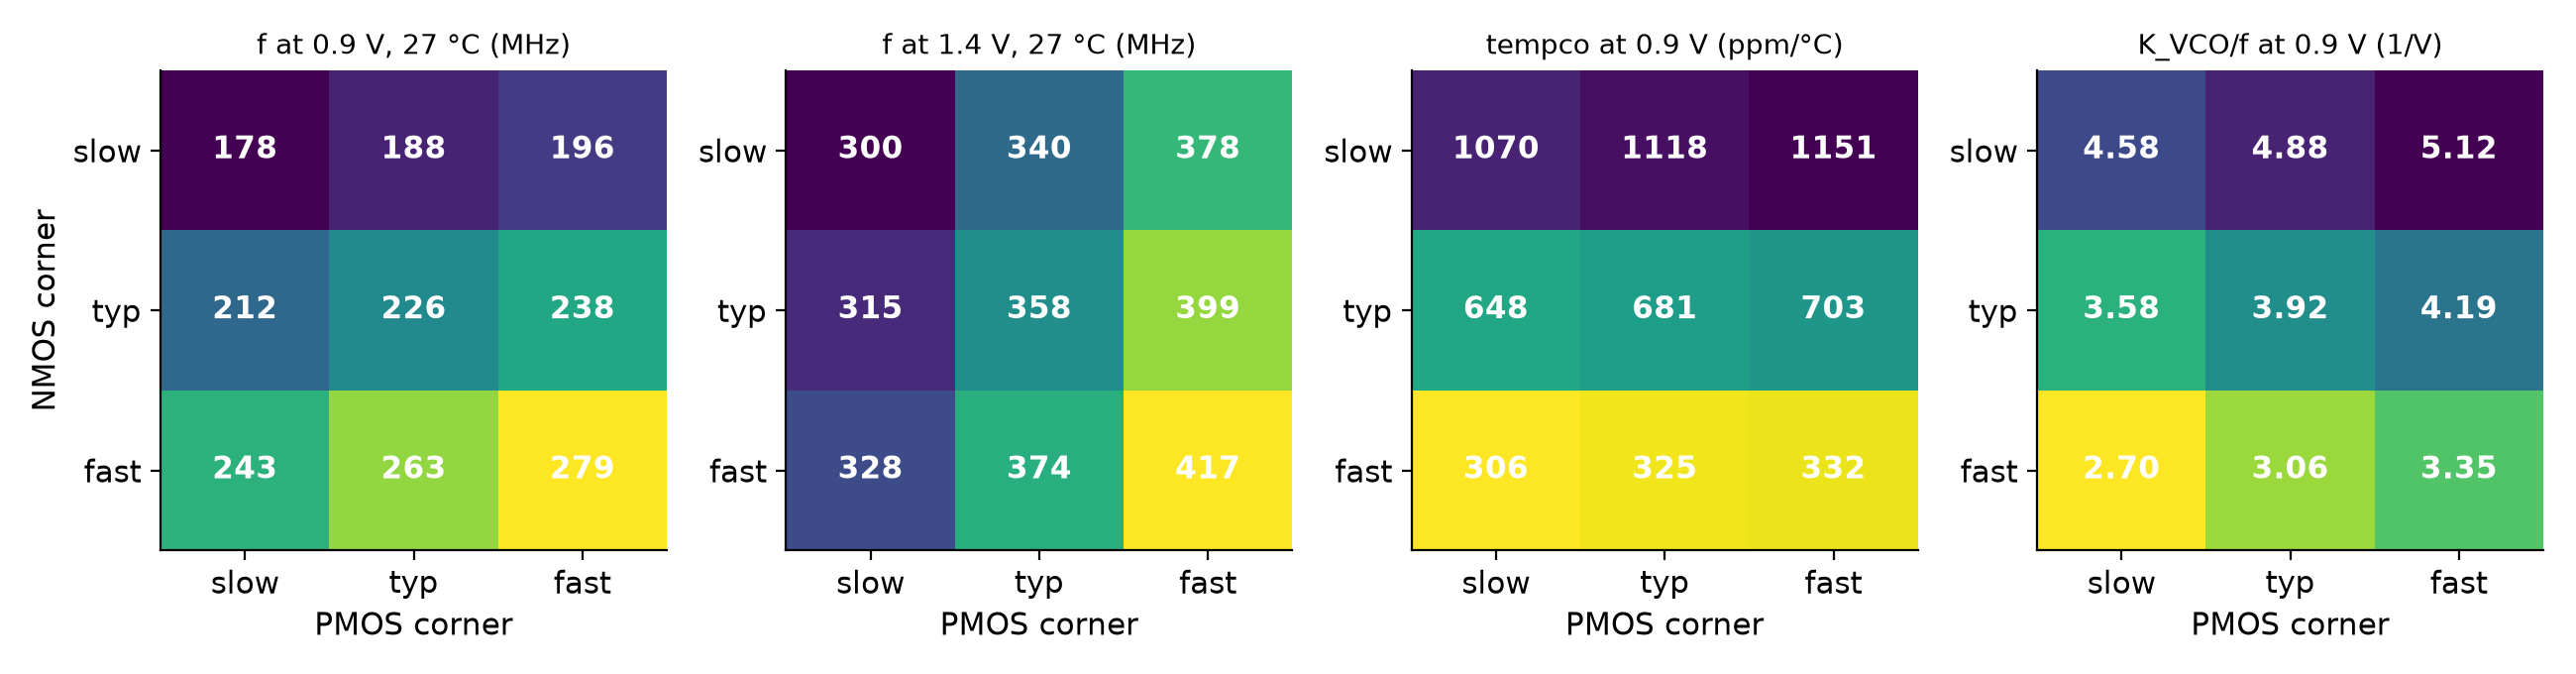
\includegraphics[width=\linewidth]{audit_factorial_maps.png}\end{center}
\figread{four heatmaps; rows are the NMOS corner (slow, typ, fast), columns the PMOS corner. Panels: $f$ at 0.9 V; $f$ at 1.4 V; tempco at 0.9 V (ppm/\degC); $K_{VCO}/f$ at 0.9 V (1/V). Colour is only relative within a panel.}
{A textbook-behaving set is smooth and monotonic: $f$ increases down the rows and right across the columns; tempco \emph{decreases} with NMOS strength. All three hold (and the checks pass automatically: 8 monotonicity checks).}
{$f(0.9\,\text{V})$: N slow 178.0/188.0/195.9; N typ 211.8/226.2/238.1; N fast 242.8/262.7/279.2 MHz. Tempco: 1070--1151 (N slow), 648--703 (N typ), 306--332 (N fast).}
{With independent N and P, the VCO behaves exactly as device physics predicts, and NMOS strength dominates at 0.9 V. Tempco range: textbook 306--1151 (3.8$\times$); PDK sf/fs 112--1399 (12.5$\times$).}
\begin{center}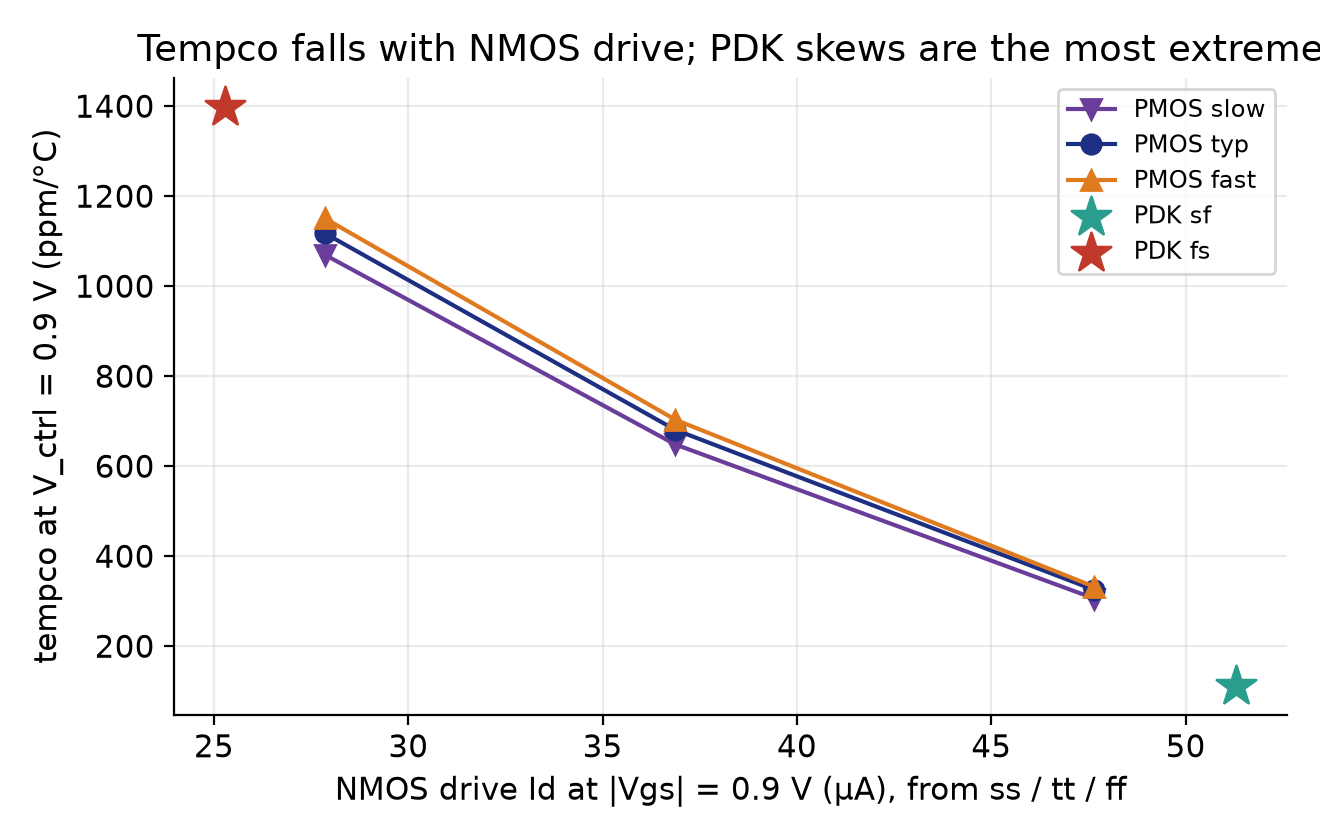
\includegraphics[width=0.52\linewidth]{audit_tempco_vs_nmos.png}\hfill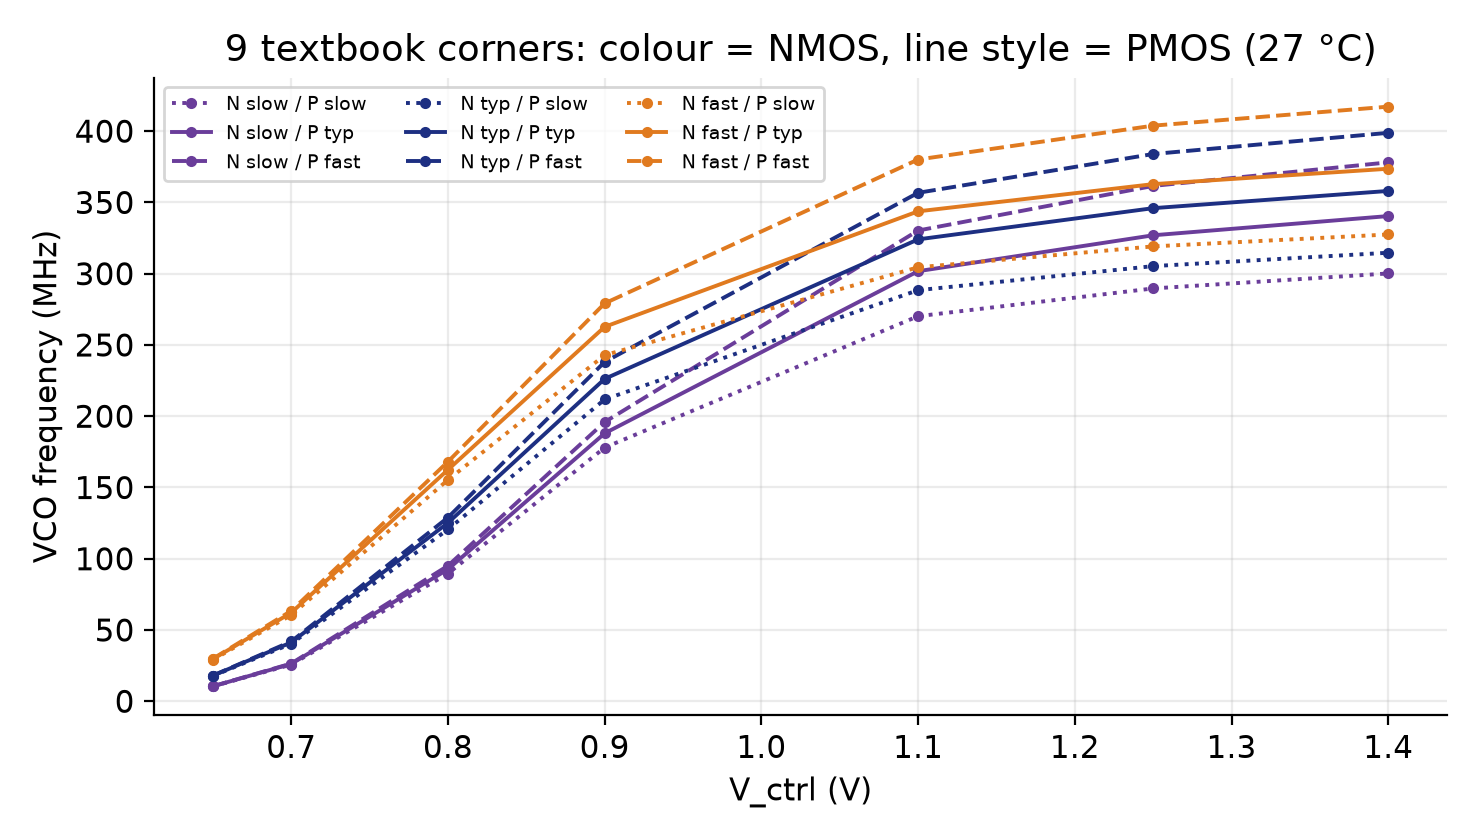
\includegraphics[width=0.46\linewidth]{audit_tuning_9corners.png}\end{center}
\figread{left: x NMOS drive current at 0.9 V ($\mu$A, from the ss/tt/ff devices), y tempco (ppm/\degC); one line per PMOS state; stars are the PDK sf/fs corners. Right: tuning curves for the 9 textbook corners (colour = NMOS, line style = PMOS).}
{Left: a straight falling line means tempco is a function of NMOS drive, which is the case. The stars lie on the extension of that trend, further out than ss/ff. Right: the colour groups (NMOS) separate more than the line styles (PMOS) at 0.9 V; they cross over at higher $V_{ctrl}$.}
{Tempco 1070 at 28 $\mu$A down to about 325 at 47.7 $\mu$A; PDK fs 1399 at 25.3 $\mu$A, PDK sf 112 at 51.3 $\mu$A.}
{The star points confirm the extremes are explained by NMOS drive, not by a bug.}

\subsection{Physics sanity checks (all pass)}
\begin{itemize}
\item $V_{th}$ falls with temperature: $-0.78$ mV/\degC\ (NMOS), $-1.1$ mV/\degC\ (PMOS); textbook range $-0.5$ to $-3$.
\item Drain current at 1.8 V \emph{falls} with temperature ($-30\%$ over 125\,\degC, mobility dominates); at 0.9 V it \emph{rises} ($+14\%$, $V_{th}$ drop dominates). So the 0.9 V bias is below the zero-tempco point, which is why $f$ rises with $T$. At $V_{ctrl}=1.4$ V (more overdrive) the tempco is $-816$ ppm/\degC: the sign flips.
\item Supply current is proportional to frequency ($C\approx27$--30 fF per node) in every corner.
\item All ordering checks pass, except that the PDK sf/fs \emph{tempcos} are outside [ff, ss] = [332, 1070] (expected, see above); their \emph{frequencies} are inside the ss--ff envelope at 0.9 and 1.4 V.
\item Closed-loop lock voltage equals the open-loop voltage for 226.2 MHz within 0.2 mV at all 11 corners (Section~\ref{sec:loop}).
\end{itemize}
\begin{careful}
Two PDK model sets exist (legacy per-corner files, which our ngspice library uses, and ``continuous'' parameter files where the skew shifts are $\pm27$ mV vs $\pm15$ mV for ss/ff). The qualitative story is the same. We cannot claim to know the foundry's intent; we report measured behaviour.
\end{careful}

%=====================================================================
\section{VCO characterisation and the tempco mechanism}
\begin{itemize}
\item \textbf{Grid:} 5 PDK corners $\times$ 6 temperatures ($-40,-20,0,27,50,85$\,\degC) at $V_{ctrl}=0.9$ V, plus the $3\times3$ textbook set.
\item \textbf{Mechanism (supported interpretation):} $V_{ctrl}$ drives the NMOS starving gate; at 0.9 V its overdrive is small. When temperature rises, $V_{th}$ drops by $\sim$0.8 mV/\degC\ (more current) and mobility drops (less current). At low overdrive the $V_{th}$ effect wins, so current and frequency rise. Less overdrive $\Rightarrow$ stronger positive tempco; this is exactly the corner ranking. At 1.4 V mobility wins and the tempco is negative. A separate isolation experiment was not run, so we call this a well-supported interpretation, not a proof.
\item \textbf{Why ``NMOS drive'' and not ``N/P balance'':} the earlier explanation (mismatched corners balancing the current sources) was wrong; see Section~\ref{sec:corr}.
\end{itemize}

%=====================================================================
\section{The compensation network and how the fit works}
\begin{center}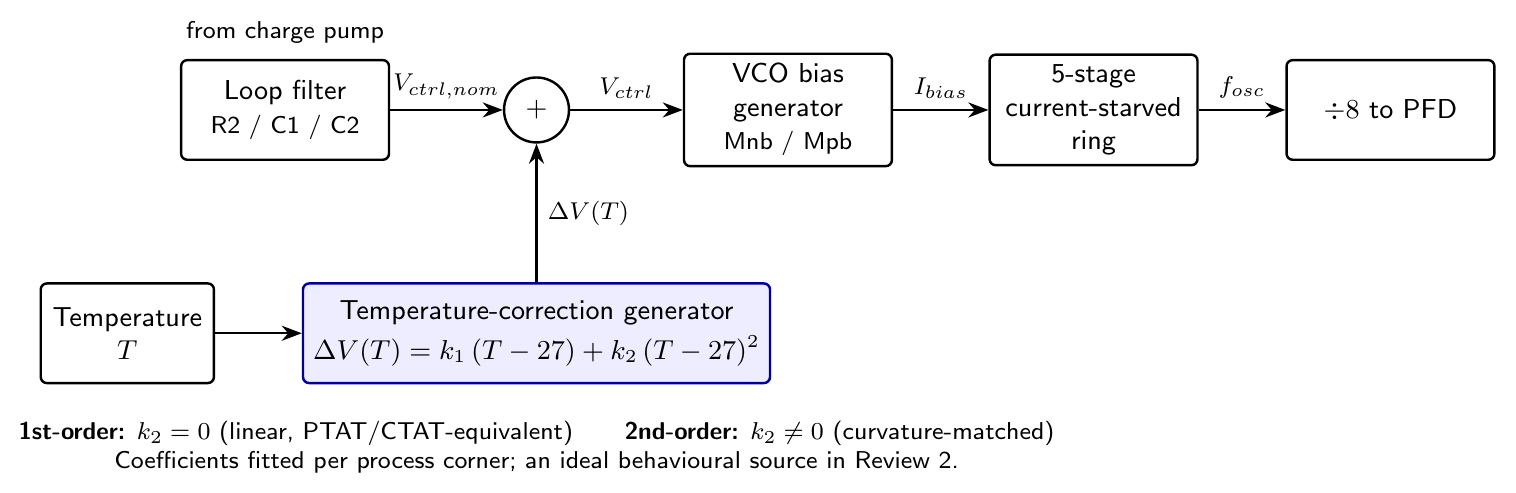
\includegraphics[width=0.9\linewidth]{compensation_arch.png}\end{center}
\[ V_{ctrl,eff}=V_{ctrl}+k_1(T-27)+k_2(T-27)^2 \]
\begin{itemize}
\item \textbf{Implementation:} an ideal behavioural voltage source (ngspice B-source reading the simulator temperature). It is \emph{not} transistors; in silicon a PTAT/CTAT current generator plus a squarer would do this. The compensation is nominal (no mismatch).
\item \textbf{How the new fit works} (\texttt{scripts/comp\_factorial.py}): (1) measure $f(T,V)$ at $V=0.85/0.9/0.95$ V for 6 temperatures; (2) at each temperature solve for the exact voltage shift $\Delta V^*(T)$ that restores $f(27\,\text{\degC})$; (3) least-squares fit $k_1$ (1st order: $k_1(T-27)$ only) and $k_1,k_2$ (2nd order); (4) \emph{verify} by simulating the compensated VCO at the 6 fit temperatures and at 4 held-out temperatures. This uses the true local sensitivity of the circuit, not a guess for $K_{VCO}$.
\item \textbf{tt coefficients:} 1st-order-only fit $k_1=-1.623\times10^{-4}$ V/\degC; 2nd-order fit $k_1=-1.543\times10^{-4}$ V/\degC, $k_2=4.18\times10^{-7}$ V/\degC$^2$. Because frequency rises with $T$, $k_1<0$ (it lowers the control voltage when hot).
\end{itemize}
\textbf{Definitions.}
\begin{itemize}
\item \textbf{Span:} max $-$ min of $f$ over $-40$ to 85\,\degC, as \% of $f_{27}$.
\item \textbf{Max deviation:} largest $|f-f_{27}|/f_{27}$ over the range, in \%. The spec $\pm0.3\%$ is judged on this.
\item \textbf{Held-out:} temperatures ($-30,10,40,70$\,\degC) never used in the fit, simulated afterwards as an overfitting guard (2 coefficients, 5 independent temperature points).
\item \textbf{Compensation ratio $C$:} baseline span / 2nd-order span. Bigger is better.
\end{itemize}

\subsection{Typical corner}
\begin{center}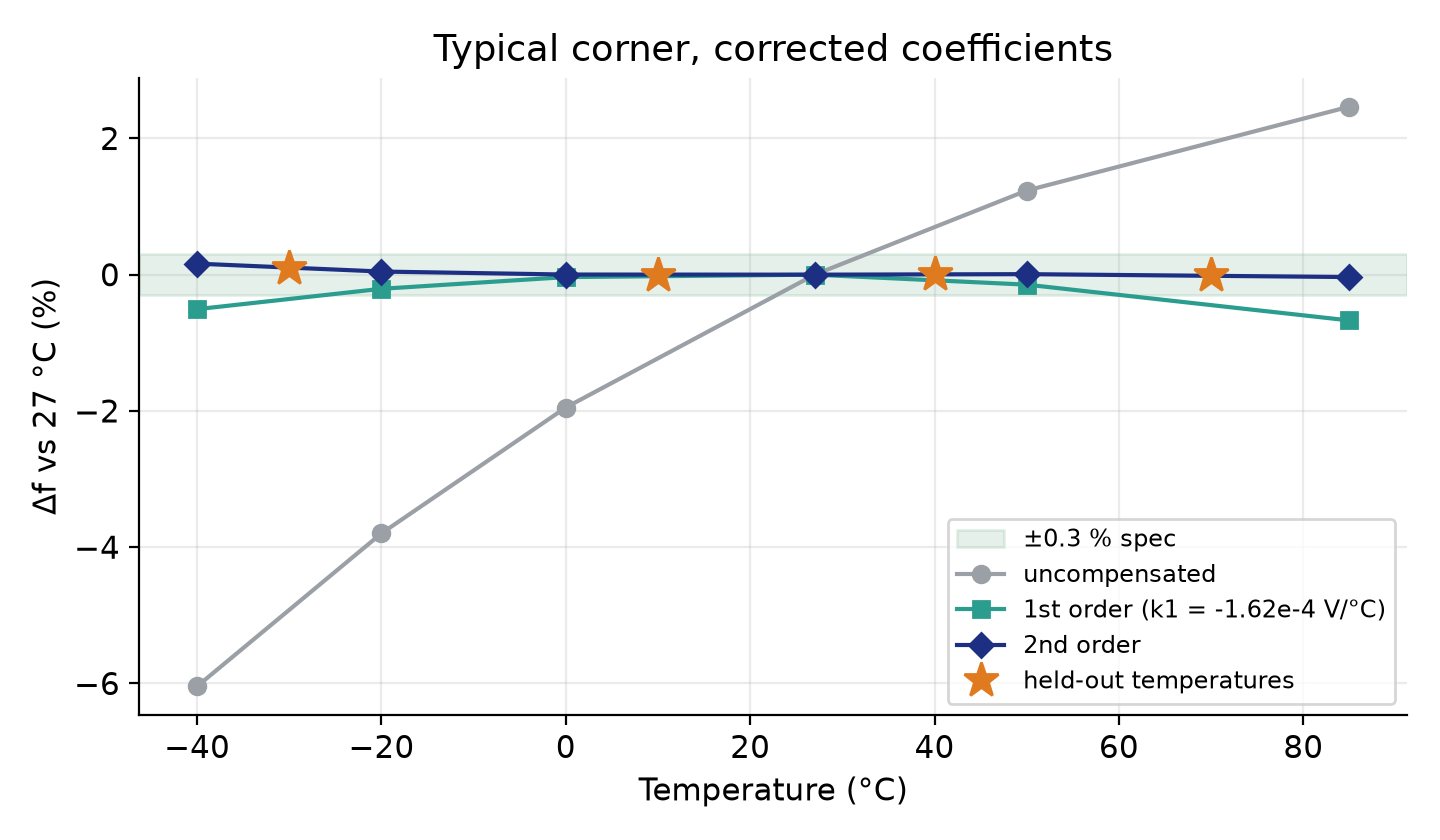
\includegraphics[width=0.7\linewidth]{final_comp_tt.png}\end{center}
\figread{x: temperature (\degC); y: frequency change relative to 27\,\degC\ (\%). Grey: uncompensated; teal squares: 1st order; navy diamonds: 2nd order; orange stars: the held-out temperatures (second-order result). Green band: $\pm0.3\%$ spec. The legend's $k_1=-1.62\times10^{-4}$ belongs to the 1st-order-only fit.}
{Good = the curve stays inside the green band. Grey leaves it ($-6\%$ to $+2.5\%$); 1st order bows out to about $-0.65\%$ at 85\,\degC; 2nd order stays in the band and the stars (never fitted) sit on the same line.}
{Span 8.51\% $\to$ 0.67\% (1st) $\to$ 0.20\% (2nd); max deviation 0.16\% (spec met); held-out max dev 0.09\%; $C=43$.}
{With correctly fitted coefficients the 2nd-order network meets spec at tt, and the held-out points show it is not overfitted.}

\subsection{All 11 corners}
\begin{center}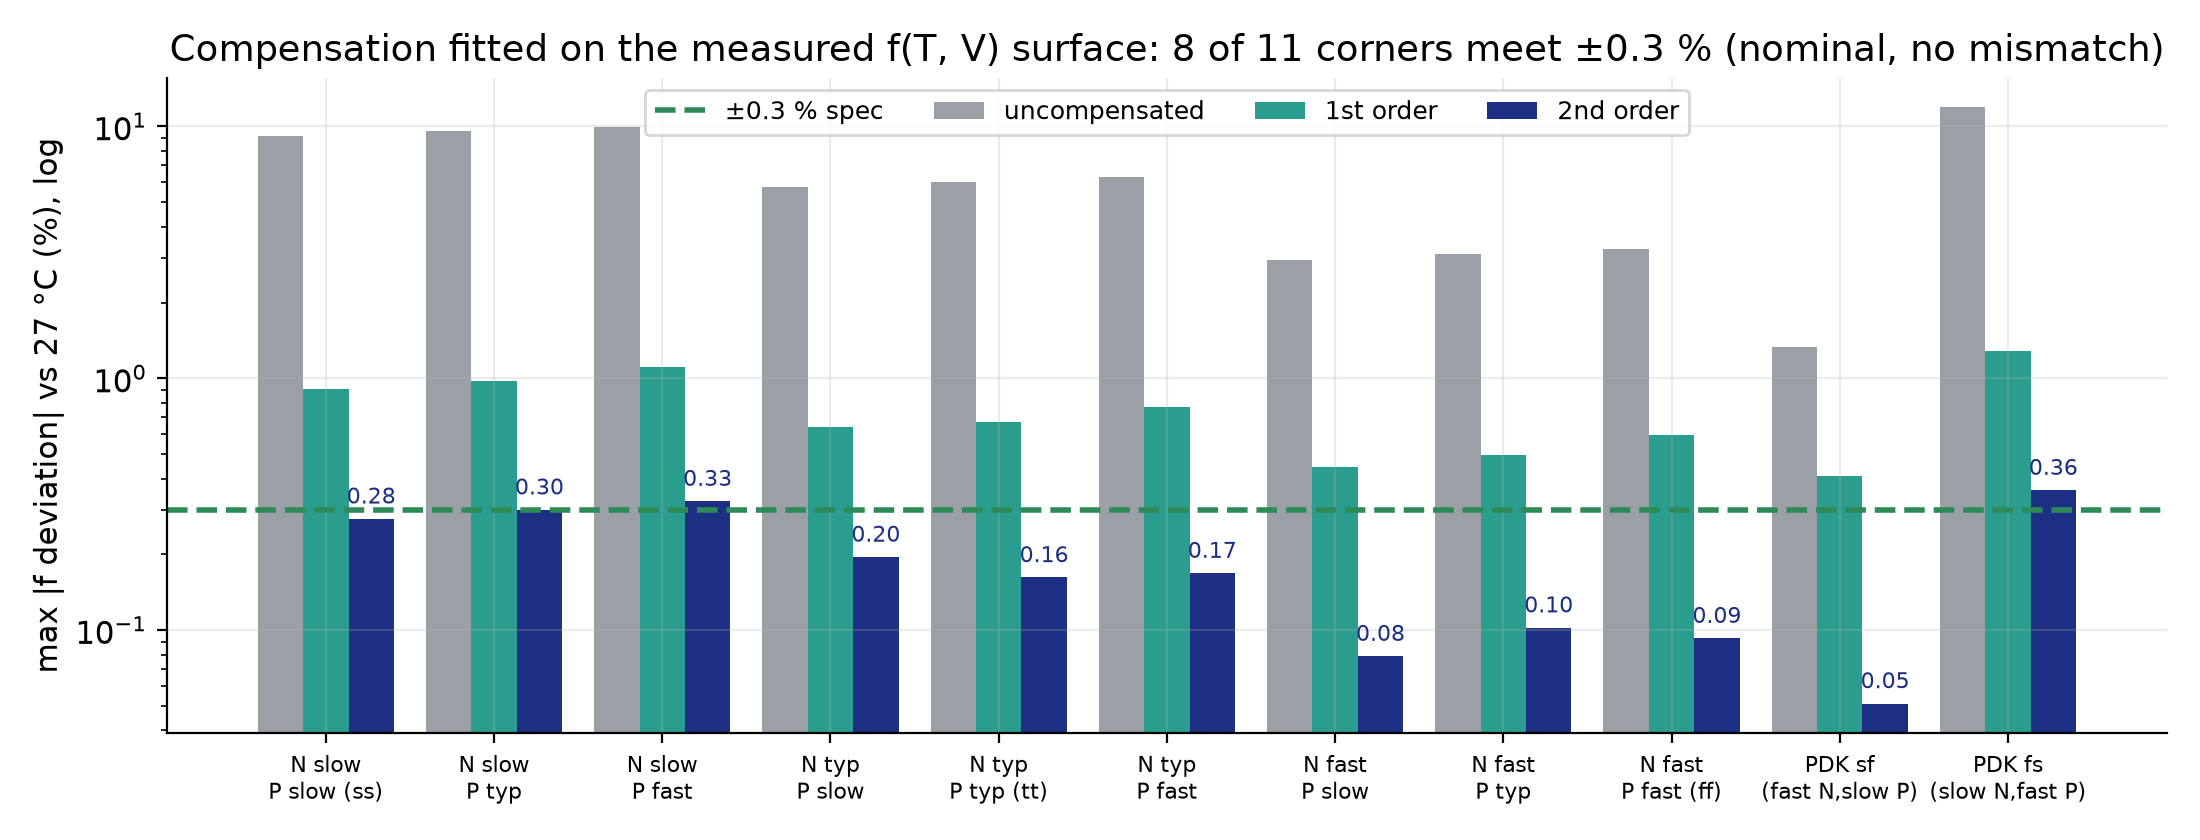
\includegraphics[width=\linewidth]{final_comp_corners.png}\end{center}
\figread{x: the 11 corners (textbook nXpY, with ss/tt/ff marked, plus PDK sf and fs); y: max $|f-f_{27}|$ in \% on a \emph{log} axis. Grey: uncompensated; teal: 1st order; navy: 2nd order (value printed). The dashed green line is the $\pm0.3\%$ spec.}
{A navy bar below the dashed line passes. Each log gridline is a factor of 10, so the grey-to-navy gap of 1--2 decades is a 30--50$\times$ improvement. Bars above the line are failures.}
{8 of 11 meet spec; the misses are N slow/P typ 0.301, N slow/P fast 0.325 and PDK fs 0.360.}
{Every corner improves by one to two orders of magnitude; the three misses are all slow-NMOS corners, where the drift is largest and the fit has the most to correct.}
\begin{center}\small\begin{tabular}{lrrrrrrl}\toprule
Corner & Base \% & 1st \% & 2nd \% & $C$ & max dev \% & held-out \% & Meets?\\\midrule
ss (nsps) & 13.37 & 0.91 & 0.35 & 38.4 & 0.277 & 0.175 & \textcolor{ok}{yes}\\
N slow/P typ & 13.97 & 0.98 & 0.38 & 37.2 & 0.301 & 0.201 & \textcolor{warn}{no}\\
N slow/P fast & 14.38 & 1.10 & 0.42 & 34.3 & 0.325 & 0.223 & \textcolor{warn}{no}\\
N typ/P slow & 8.10 & 0.64 & 0.24 & 33.6 & 0.195 & 0.109 & \textcolor{ok}{yes}\\
tt (ntpt) & 8.51 & 0.67 & 0.20 & 43.2 & 0.162 & 0.091 & \textcolor{ok}{yes}\\
N typ/P fast & 8.79 & 0.77 & 0.20 & 43.7 & 0.168 & 0.097 & \textcolor{ok}{yes}\\
N fast/P slow & 3.82 & 0.45 & 0.12 & 31.0 & 0.079 & 0.034 & \textcolor{ok}{yes}\\
N fast/P typ & 4.06 & 0.50 & 0.12 & 33.3 & 0.102 & 0.041 & \textcolor{ok}{yes}\\
ff (nfpf) & 4.15 & 0.59 & 0.11 & 37.0 & 0.093 & 0.035 & \textcolor{ok}{yes}\\
PDK sf (fast N/slow P) & 1.49 & 0.41 & 0.09 & 15.9 & 0.051 & 0.036 & \textcolor{ok}{yes}\\
PDK fs (slow N/fast P) & 17.49 & 1.29 & 0.49 & 35.8 & 0.360 & 0.251 & \textcolor{warn}{no}\\\bottomrule
\end{tabular}\end{center}
\noindent 7 of the 9 textbook corners meet spec; 8 of all 11. $C$ ranges 31--44 except PDK sf (15.9), whose baseline is already tiny. Held-out max deviation ranges 0.03--0.25\%.

\textbf{Which do not meet, and why.} N slow/P typ (0.301, borderline: it misses by 0.001 points), N slow/P fast (0.325) and PDK fs (0.360). Slow NMOS means the smallest overdrive, the largest and most curved drift (baseline spans 14--17.5\%), and a residual that a single quadratic cannot flatten to better than about 0.3--0.36\%. They are close; we do not call them ``met''.
\begin{careful}
Caveats to state yourself: the source is ideal; this is nominal (no mismatch); the fit is at $V_{ctrl}=0.9$ V; 2 coefficients are fitted to 5 temperature points (mitigated by the held-out check). Also, each corner locks at its own $V_{ctrl}$ (0.85--0.97 V), so the ideal target would be the compensation at that corner's own lock voltage (future work).
\end{careful}

%=====================================================================
\section{Monte Carlo, $n=72$}
\begin{center}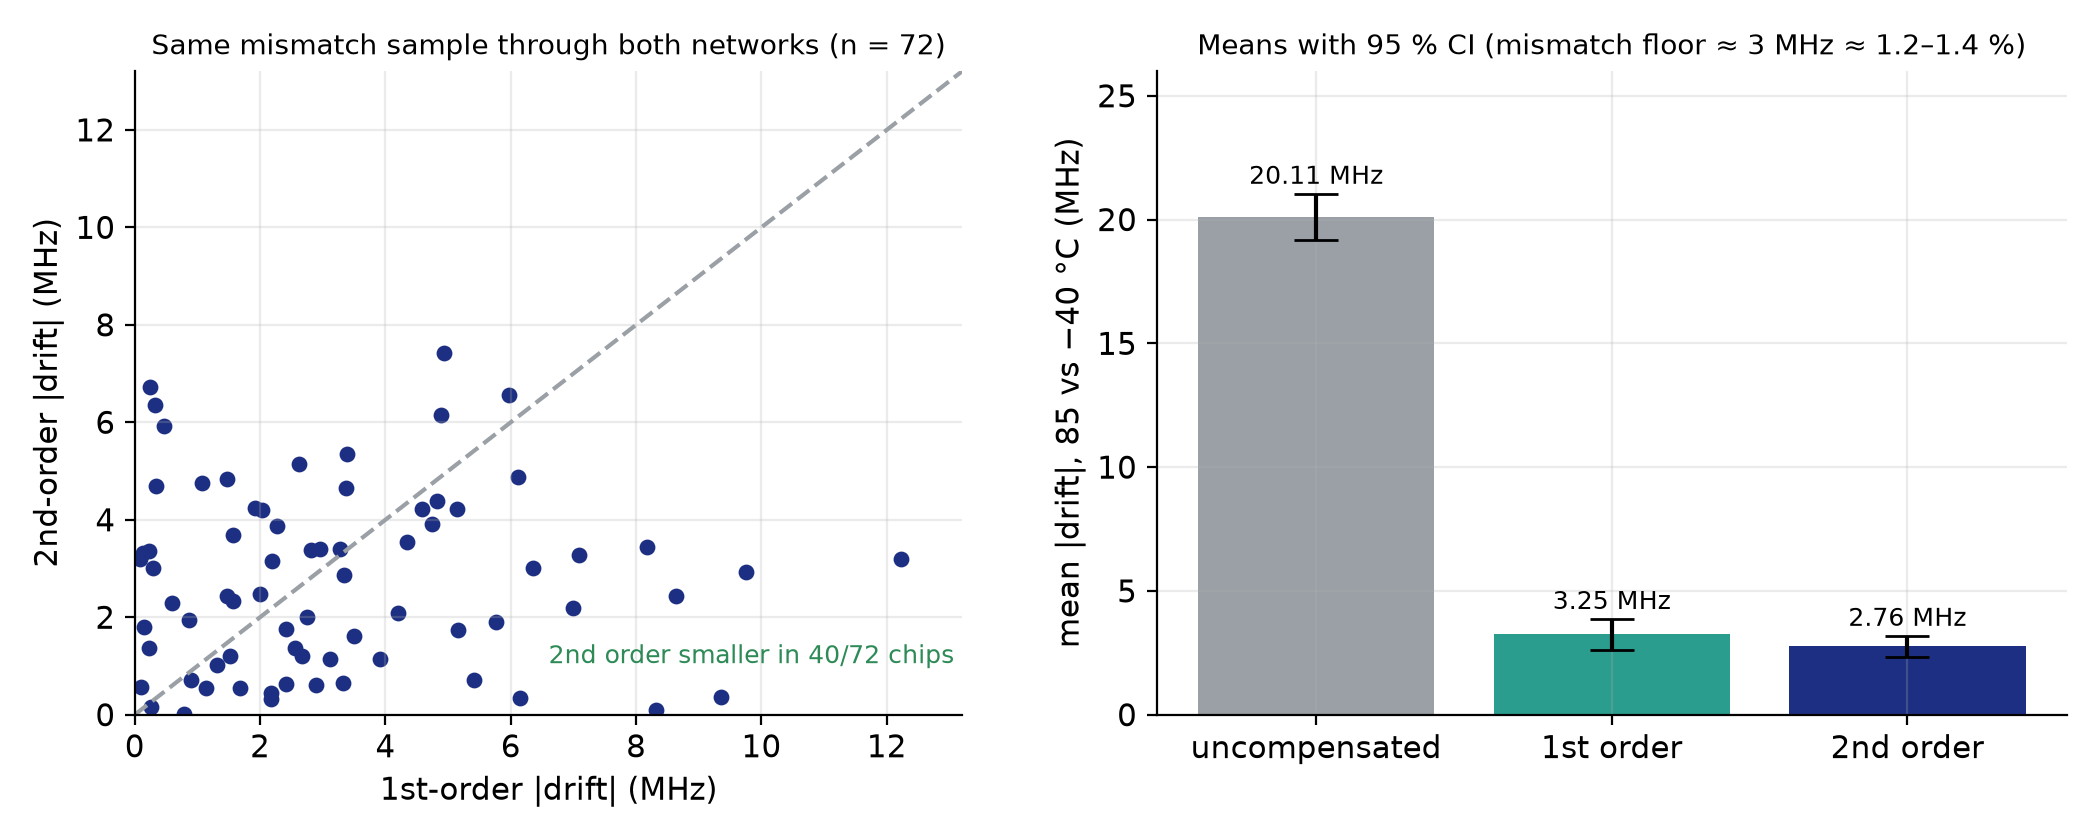
\includegraphics[width=\linewidth]{final_mc.png}\end{center}
\figread{Left: each dot is one virtual chip (one random mismatch seed at tt). x: its $|$drift$|=|f(85)-f(-40)|$ with the 1st-order network (MHz); y: the same chip with the 2nd-order network. Dashed line: equal. Right: bar chart of the mean $|$drift$|$ with 95\% confidence intervals.}
{Left: dots \emph{below} the dashed line are chips where 2nd order is better. A clear win would put almost all dots below it; here they are scattered on both sides (40 of 72 below). Right: a good result is a low bar with a small interval; the compensated bars are far below the grey one but overlap each other.}
{Mean $|$drift$|$: 20.11 MHz [19.18, 21.04] uncompensated; 3.25 MHz [2.63, 3.87] 1st order; 2.76 MHz [2.33, 3.19] 2nd order.}
{Compensation works on mismatched chips (72/72 improve), but 2nd order is not distinguishable from 1st order. The remaining 3 MHz is a mismatch floor.}

\subsection{What a paired test is, in plain language}
Each seed is a virtual chip with its own random transistor mismatch. Chips differ a lot from one another, which would drown a small difference between two networks. \emph{Pairing} means we run the \emph{same} chip through both networks and look only at the per-chip difference, so chip-to-chip variation cancels. We then ask: is the mean of those differences distinguishable from zero? The 95\% confidence interval (CI) is the range likely to contain the true mean difference; if it contains 0, the effect is not significant. The paired $t$-test assumes roughly normal differences; Wilcoxon signed-rank uses ranks only and does not. We report both; they agree. The metric is $|$drift$|$ (not signed drift; see Section~\ref{sec:corr}).

\subsection{Results}
\begin{center}\small\begin{tabular}{lrll}\toprule
Comparison & Mean reduction (MHz) & 95\% CI & Significant?\\\midrule
Baseline $\to$ 1st order & 16.86 & [15.57, 18.16] & yes ($t$ and Wilcoxon), better in 71/72\\
Baseline $\to$ 2nd order & 17.35 & [16.37, 18.34] & yes (both), better in 72/72\\
1st $\to$ 2nd order & 0.49 & [$-0.26$, 1.24] & \textbf{no} (both), 2nd smaller in 40/72\\\bottomrule
\end{tabular}\end{center}
\subsection{The mismatch floor, and why this is an honest finding}
Nominally the residual is only 0.2--0.7\%. With mismatch each chip has its own drift curve, but we apply one global correction fitted to the nominal chip. What cannot be removed is each chip's own deviation: about 3 MHz, which is 1.2--1.4\% of 226 MHz. Signed-drift standard deviation is 4.1 MHz (1st) and 3.3 MHz (2nd): the spread across chips, not the average, is the problem. The 2nd-order term refines the \emph{average} shape; but the error per chip is dominated by mismatch, so improving the mean shape by 0.2--0.5\% does not show up. The CI for 1st vs 2nd order includes zero, so we cannot claim 2nd order helps under mismatch. This is the correct conclusion with correctly fitted coefficients. Getting to $\pm0.3\%$ across chips would need a per-chip trim (future work).

%=====================================================================
\section{Closed loop}\label{sec:loop}
\subsection{Loop dynamics, found, fixed, verified}
\begin{itemize}
\item The loop is a second-order system with natural frequency $\omega_n^2=I_{cp}K_{VCO,rad}/(2\pi NC_1)$ and damping $\zeta=R_2C_1\omega_n/2$. The $1/(2\pi)$ comes from the PFD/charge-pump gain ($I_{cp}/2\pi$ amps per radian of phase error). Review 1 dropped it.
\item With the measured $K_{VCO}=887$ MHz/V and the original $R_2=1.7$ k$\Omega$: $f_n\approx0.91$ MHz, $\zeta\approx0.33$ (underdamped, rings). Review 1 had claimed $\zeta=0.72$.
\item $\zeta$ depends on $R_2$ at fixed $f_n$, so we raised $R_2$ to 3.6 k$\Omega$: $f_n\approx0.91$ MHz, $\zeta\approx0.70$, phase margin about 65--70\degree\ \emph{by the $100\zeta$ rule of thumb}, not a Bode plot.
\end{itemize}
\begin{center}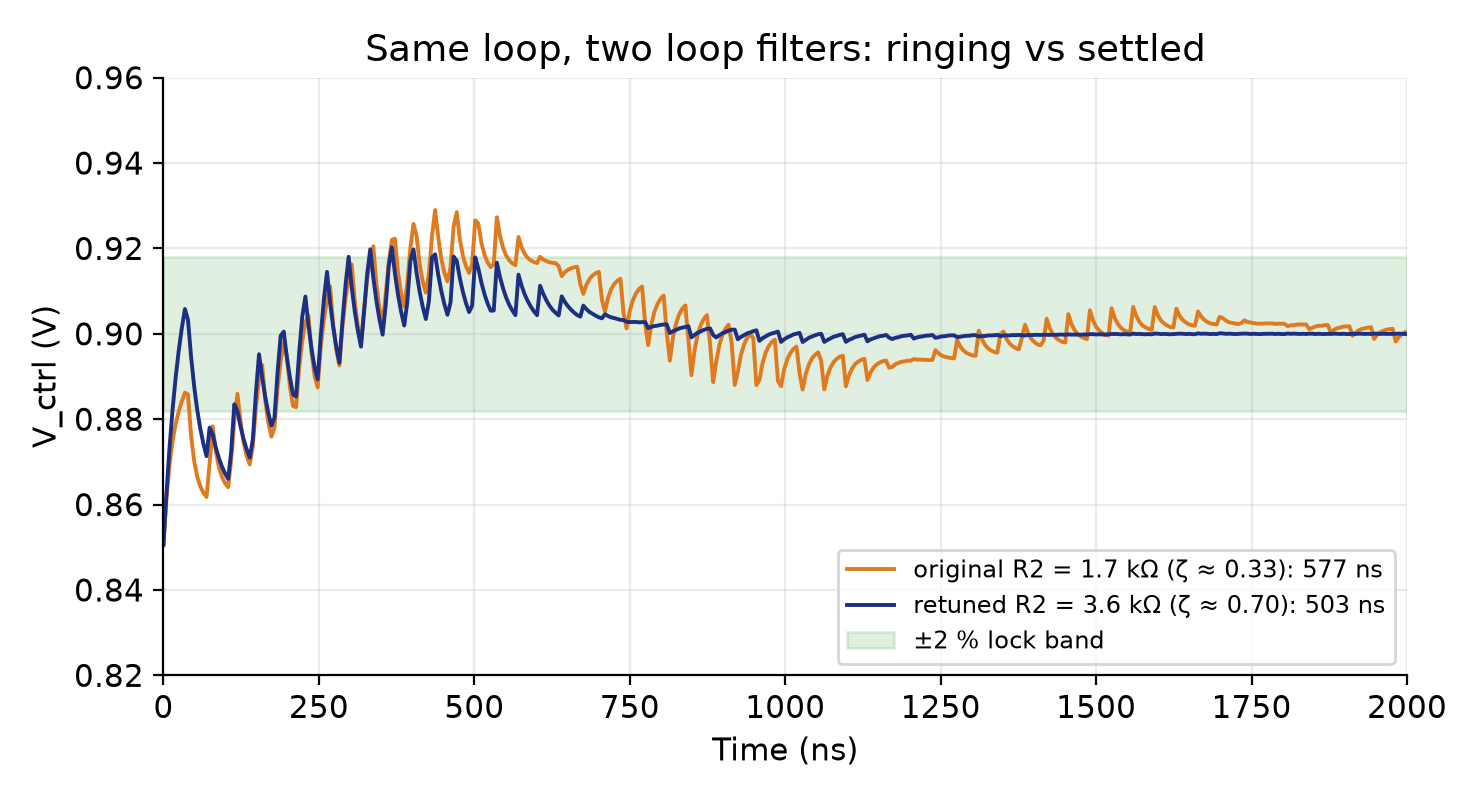
\includegraphics[width=0.7\linewidth]{lock_compare.png}\end{center}
\figread{x: time (ns); y: $V_{ctrl}$ (V), tt, 27\,\degC, coarse start at 0.85 V. Orange: original filter; navy: retuned. Green band: $\pm2\%$ of the final 0.9 V, the lock definition.}
{Good = enter the band and stay, with small ripple. Orange keeps ringing up to 2\,$\mu$s; navy settles smoothly. The sawtooth is the per-cycle charge-pump pulses.}
{Lock 577 $\to$ 503 ns; ripple 8.6 $\to$ 0.35 mV; final frequency error 0.78\% $\to$ 0.008\%; peak $V_{ctrl}$ 0.930 $\to$ 0.922 V.}
{The retune removed the ringing; only $R_2=1.7$, 3.0 and 3.6 k$\Omega$ were simulated at transistor level, so 3.6 is not claimed optimal.}

\subsection{Cold start}
\begin{center}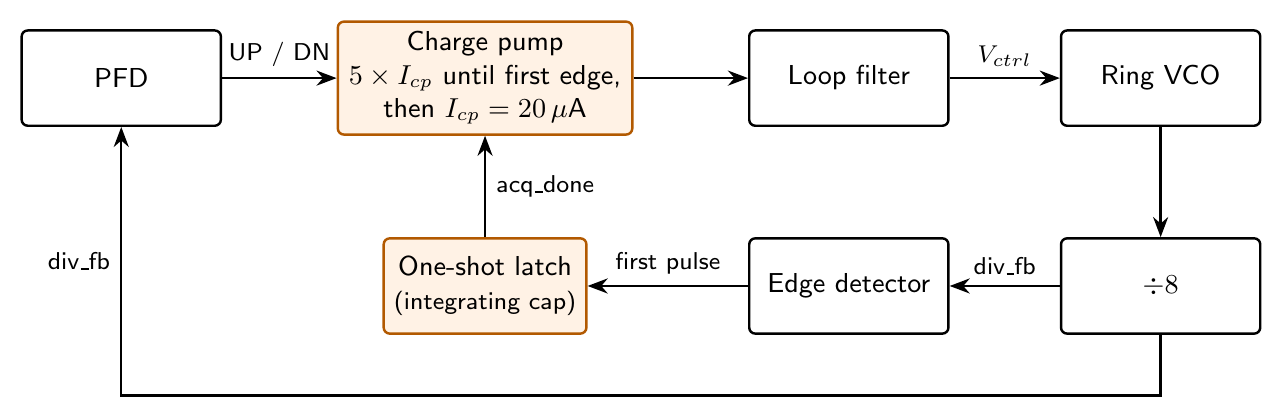
\includegraphics[width=0.62\linewidth]{acq_boost.png}\end{center}
At 0 V the VCO is nearly off, so the divided clock is absent and the nominal 20\,$\mu$A pump is too slow. The fix: run the charge pump at $5\times I_{cp}$ until the divider produces its first edge, then drop to 20\,$\mu$A. This is done by an edge detector feeding a one-shot latch. The price of the retune is that the cold start became slower (839 ns with the original filter $\to$ 1351 ns at tt); both are inside 2\,$\mu$s.
\begin{center}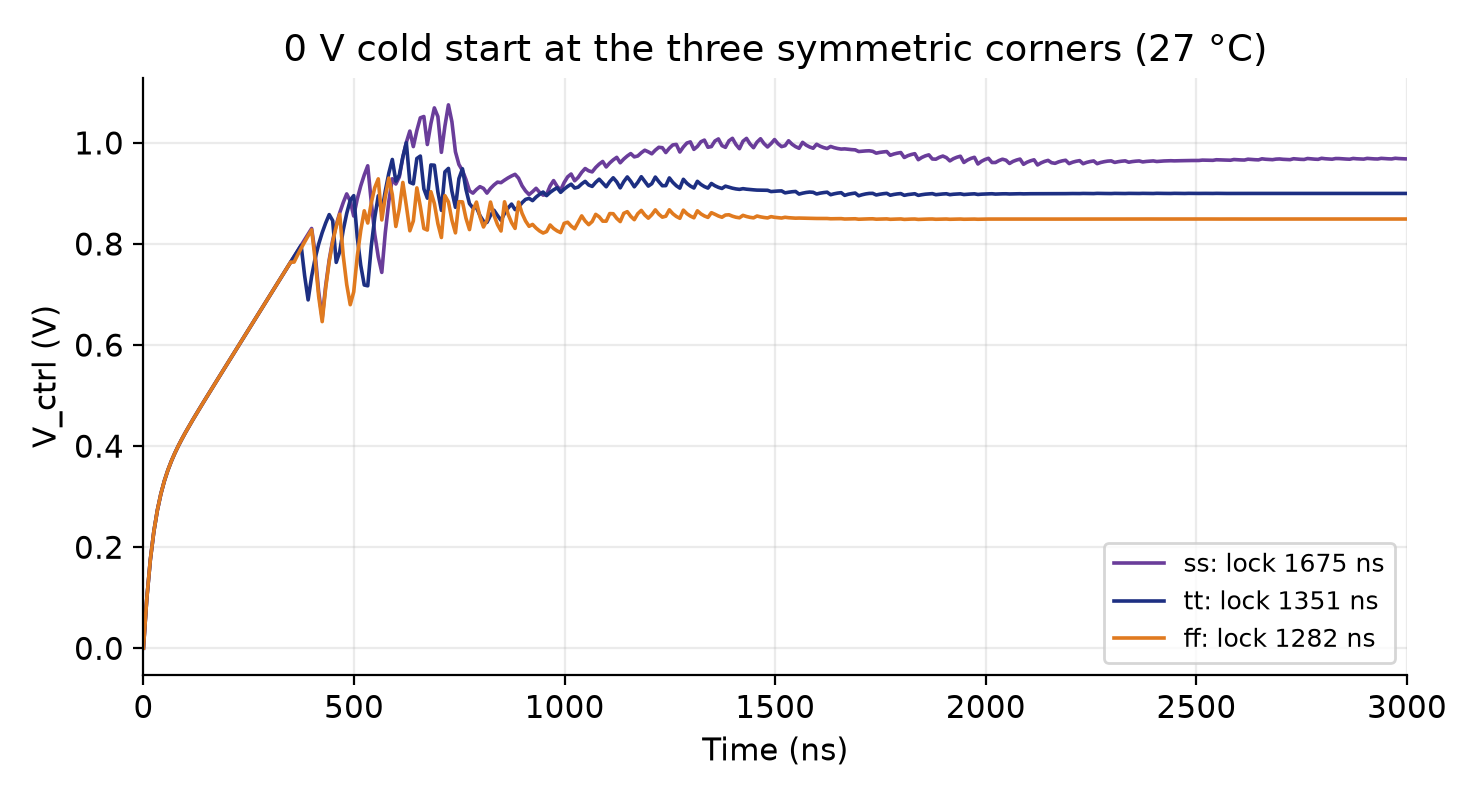
\includegraphics[width=0.7\linewidth]{final_cold_traces.png}\end{center}
\figread{x: time (ns); y: $V_{ctrl}$ (V); true 0 V start at 27\,\degC\ for ss (purple), tt (navy), ff (orange).}
{Good = a fast monotonic climb, a limited overshoot, and a flat settled value. The three curves rise together for the first 350 ns (the boosted charge pump), then ring while the loop captures phase, then settle at different final voltages.}
{Lock 1675 ns (ss), 1351 ns (tt), 1282 ns (ff); settled $V_{ctrl}$ 0.968, 0.900, 0.849 V.}
{The boost drives $V_{ctrl}$ through the dead region quickly; the loop then locks inside spec at every corner shown. ss is slowest because it needs the highest $V_{ctrl}$.}

\subsection{Lock across 11 corners}
\begin{center}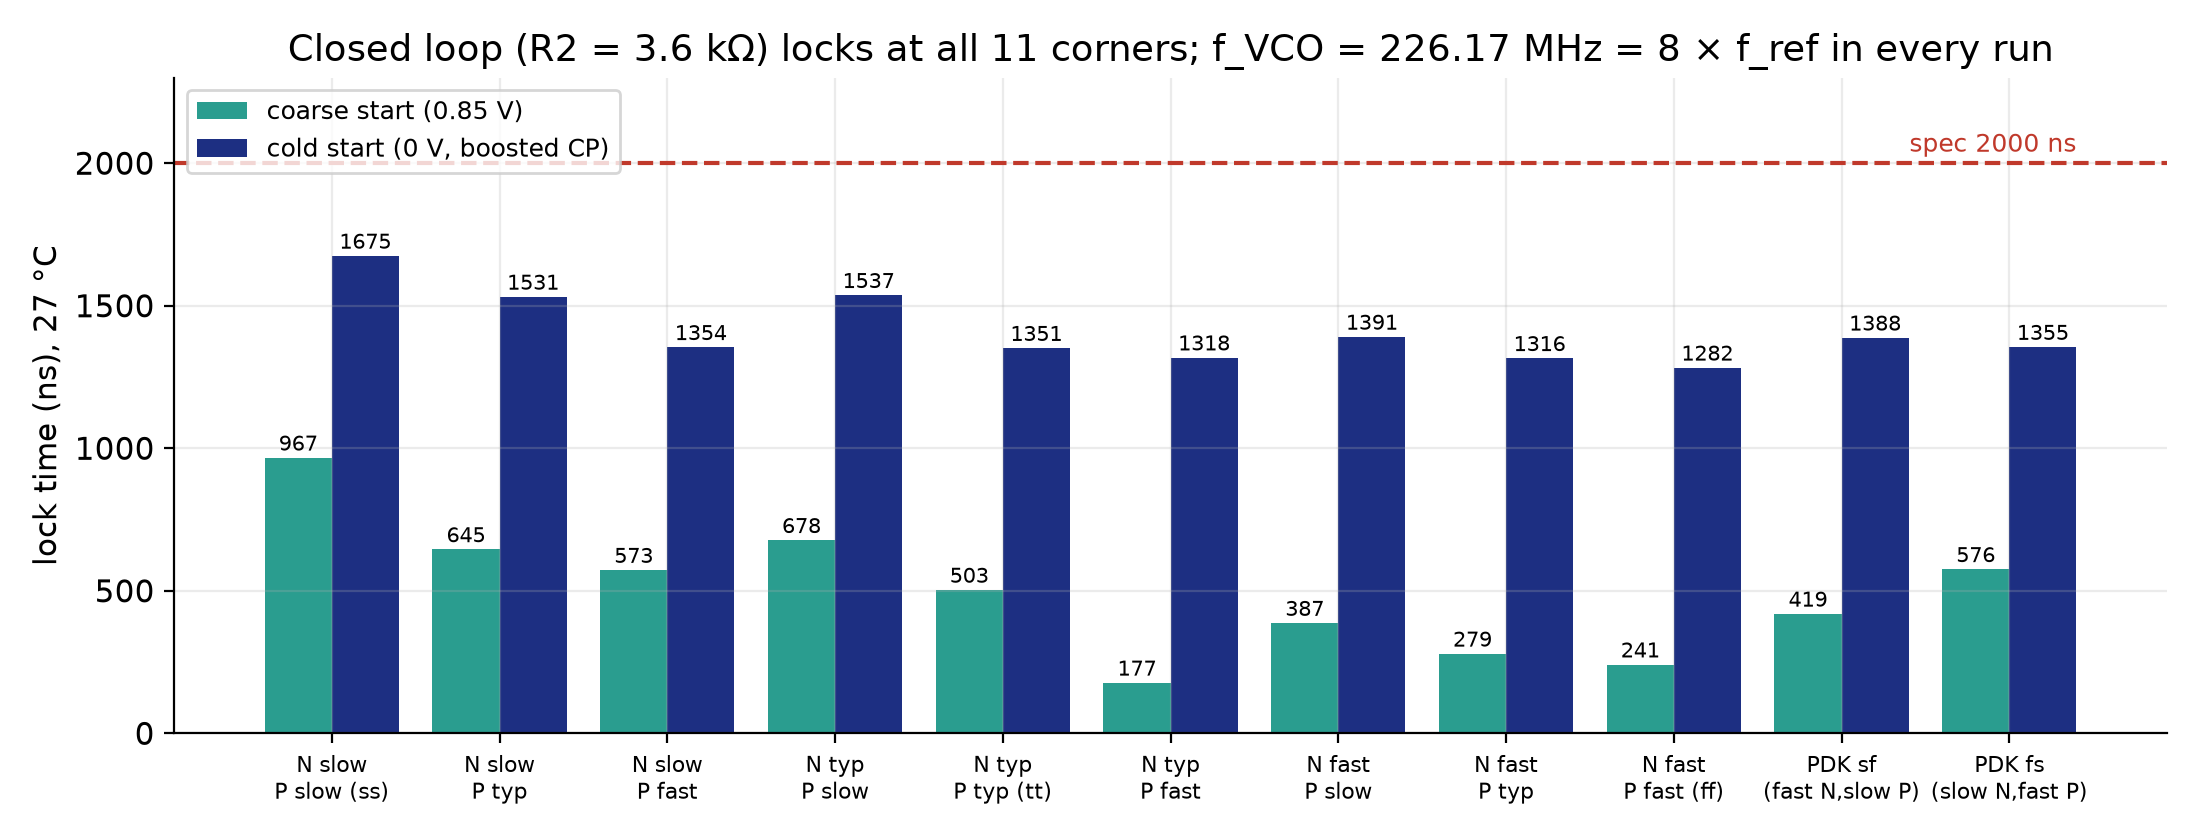
\includegraphics[width=\linewidth]{final_lock_corners.png}\end{center}
\figread{x: the 11 corners; y: lock time (ns) at 27\,\degC. Teal: coarse start (0.85 V). Navy: cold start from 0 V with boosted charge pump. Red dashed line: 2000 ns spec.}
{A bar below the red line passes; they all do at 27\,\degC. The title notes the output frequency: 226.17 MHz = $8\times f_{ref}$ in every run.}
{Coarse: 177--967 ns (ss slowest 967). Cold: 1282--1675 ns. Ripple $\le0.8$ mV, all runs settled, $f_{VCO}=226.17$ MHz ($-0.01\%$, the crossing-detector bias).}
{The same loop locks across all process corners, with comfortable margin at 27\,\degC.}
\begin{center}\small\begin{tabular}{lrrr}\toprule
Corner & Coarse (ns) & Cold (ns) & Lock $V_{ctrl}$ (V)\\\midrule
ss (nsps) & 967 & 1675 & 0.968\\ N slow/P typ & 645 & 1531 & 0.944\\ N slow/P fast & 573 & 1354 & 0.930\\
N typ/P slow & 678 & 1537 & 0.920\\ tt (ntpt) & 503 & 1351 & 0.900\\ N typ/P fast & 177 & 1318 & 0.888\\
N fast/P slow & 387 & 1391 & 0.877\\ N fast/P typ & 279 & 1316 & 0.860\\ ff (nfpf) & 241 & 1283 & 0.849\\
PDK sf & 419 & 1388 & 0.869\\ PDK fs & 576 & 1355 & 0.942\\\bottomrule
\end{tabular}\end{center}

\subsection{Temperature, and the ss/85\,\degC\ miss}
\begin{center}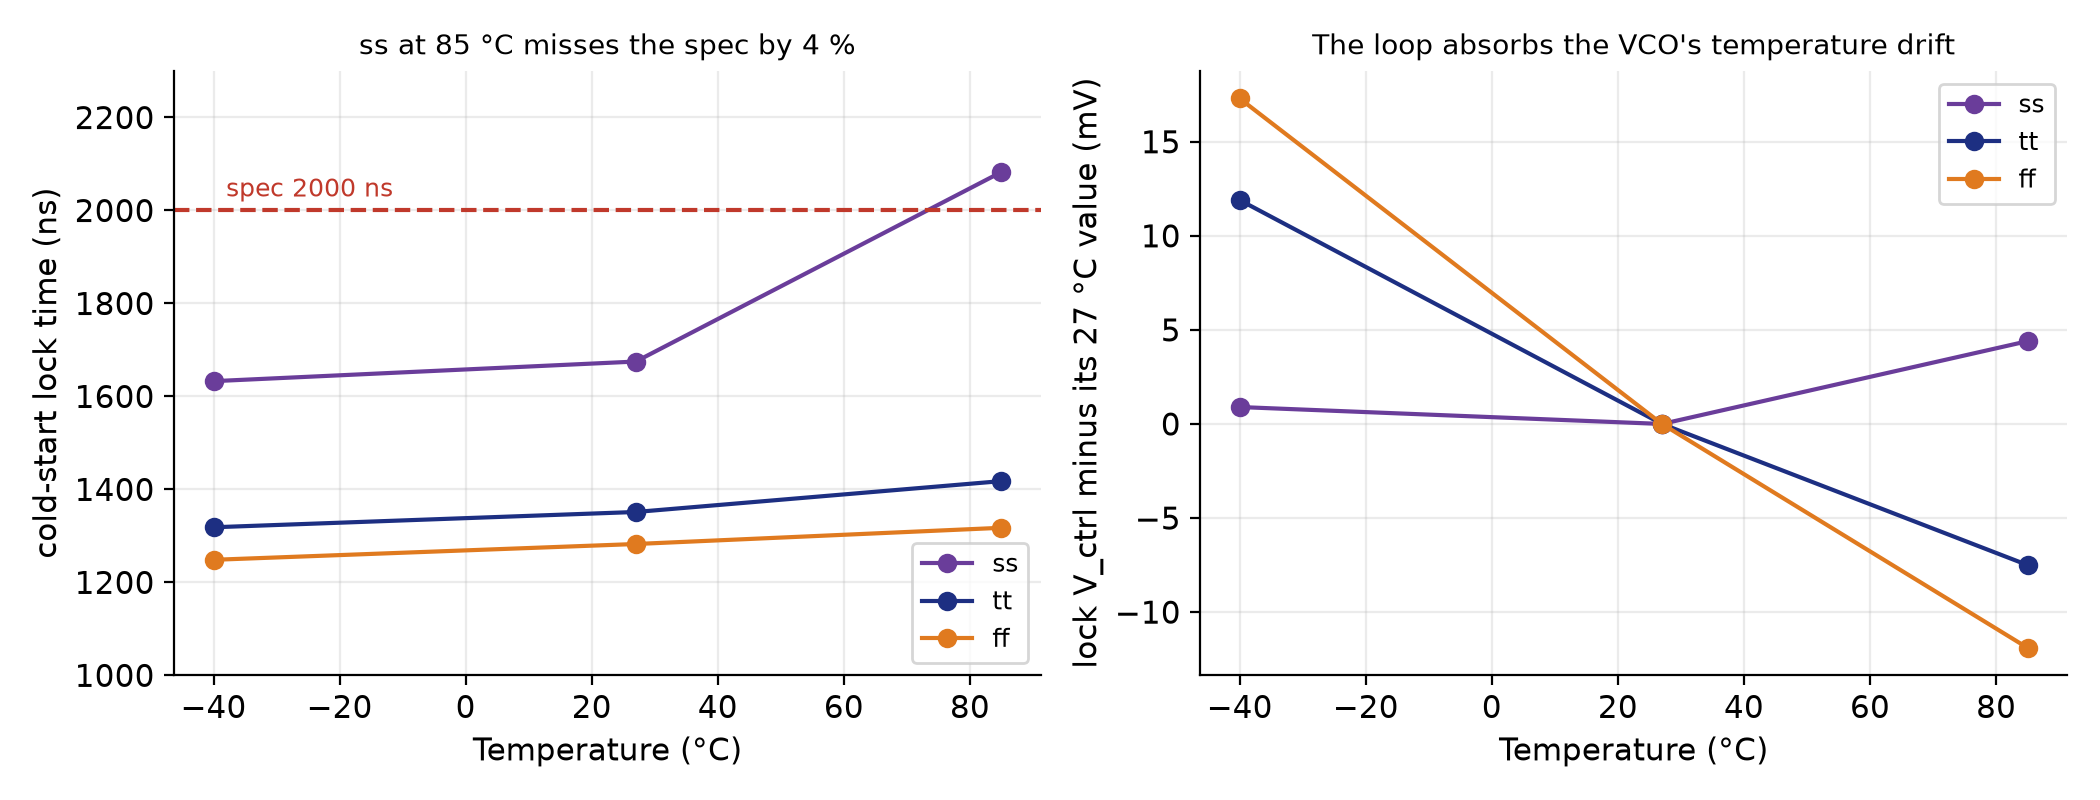
\includegraphics[width=\linewidth]{final_lock_temp.png}\end{center}
\figread{Left: x temperature (\degC); y cold-start lock time (ns) for ss, tt, ff; red dashed = 2000 ns spec. Right: x temperature; y change in the locked $V_{ctrl}$ relative to its 27\,\degC\ value (mV).}
{Left: any point above the red line fails. Right: the loop absorbs the VCO's drift by moving $V_{ctrl}$, and a larger slope means more drift absorbed.}
{ss: $-40$\,\degC\ 1633 ns, 27\,\degC\ 1675, \textbf{85\,\degC\ 2083 ns (misses 2\,$\mu$s by 4\%)}; tt 1319/1351/1418; ff 1249/1283/1317. Locked $V_{ctrl}$ at tt: $+11.9$ mV at $-40$\,\degC, $-7.5$ mV at 85\,\degC.}
{The worst case, ss at 85\,\degC, misses the lock-time spec slightly. We report it as is; the lock frequency itself is still correct (226.11 MHz).}
\noindent In lock the PLL absorbs the VCO's tempco. At tt the lock-voltage shift ($+11.9$/$-7.5$ mV) matches the fitted compensation correction ($+12.2$/$-7.5$ mV): an independent confirmation of the compensation fit \emph{at tt}. At other corners this comparison is not valid, because the compensation was fitted at 0.9 V while each corner locks at its own voltage. Temperature runs: ss, tt and ff only, cold start; not all 11 corners at all temperatures.

\subsection{Closed-loop vs open-loop voltage check}
\begin{center}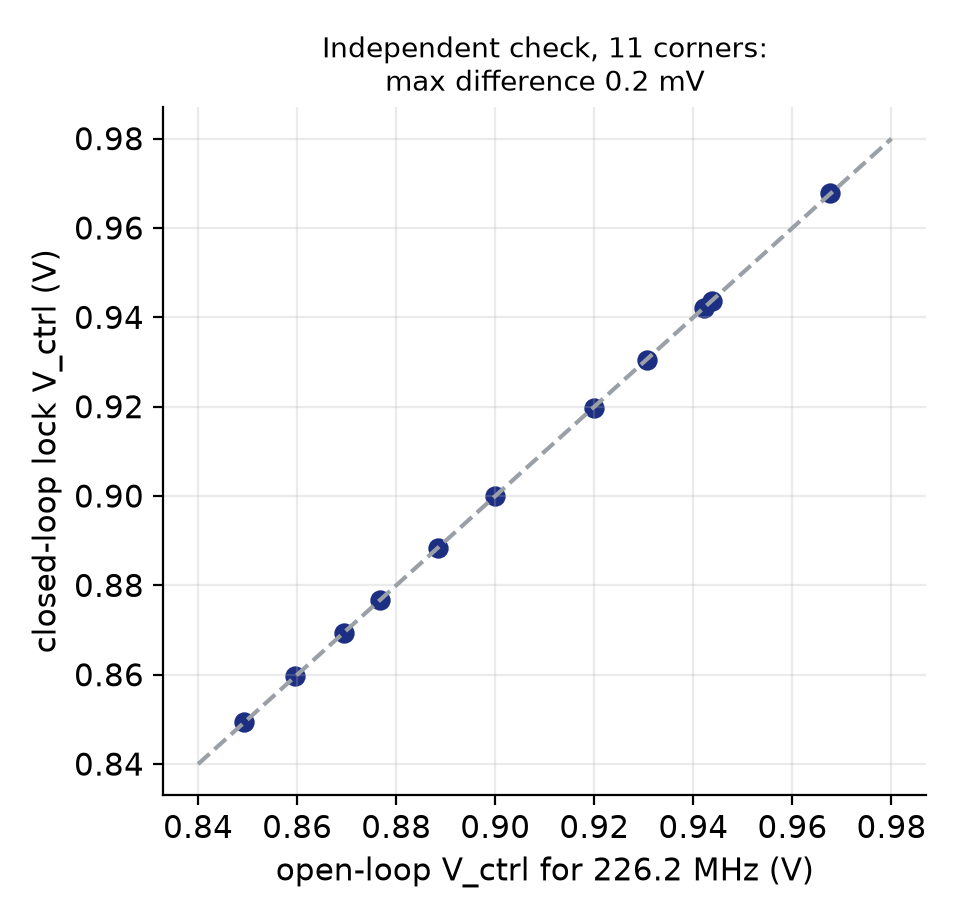
\includegraphics[width=0.45\linewidth]{final_vlock_check.png}\end{center}
\figread{x: the open-loop $V_{ctrl}$ that gives 226.2 MHz (from the free-running VCO); y: the locked $V_{ctrl}$ in the closed loop; one dot per corner; dashed 45\degree\ line = perfect agreement.}
{Good = every point on the dashed line. All 11 do.}
{Maximum difference 0.2 mV over 0.849--0.968 V.}
{Two independent simulations (open-loop VCO and closed loop) agree, so the loop is locking where the VCO actually produces 226.2 MHz.}

%=====================================================================
\section{Method, novelty and limitations}
\begin{center}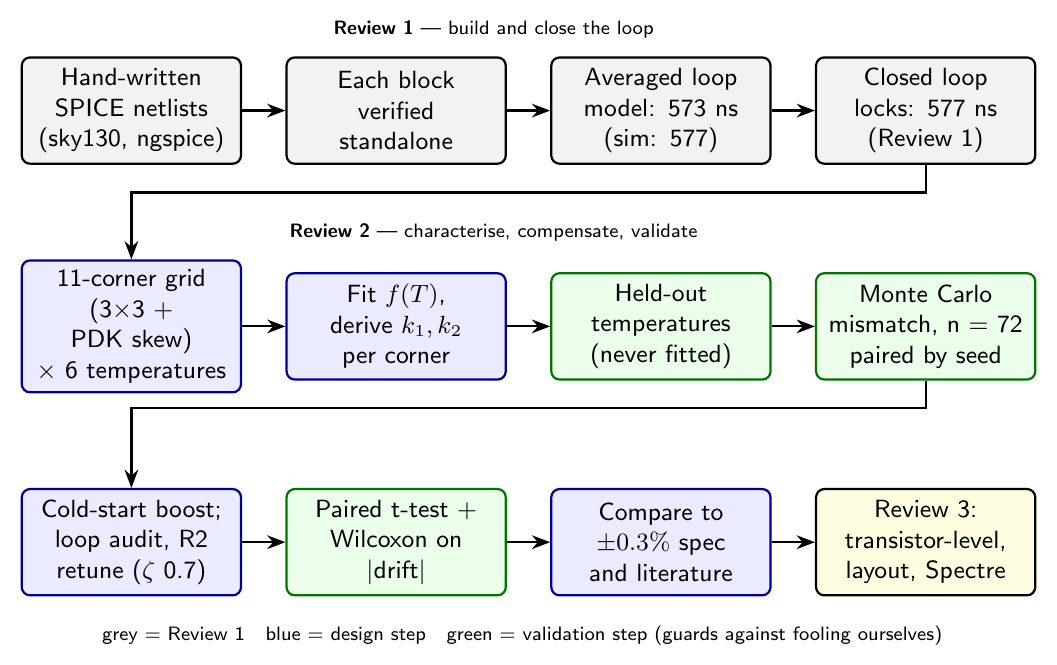
\includegraphics[width=\linewidth]{method_flow.png}\end{center}
\noindent\textit{This is the Review 1/2/3 flow diagram; its Monte Carlo box (``$n=30$'') is the Review 2 size. The final analysis uses $n=72$.}

\begin{itemize}
\item \textbf{Method:} simulate everything at transistor level in ngspice 47 with sky130B (volare commit c6d73a35); characterise $\to$ model/fit $\to$ verify on held-out data $\to$ test statistically. The green steps (held-out, paired statistics, independent checks) are there to stop us fooling ourselves.
\item \textbf{Literature and novelty:} US Patent 9,748,962 B2 (Infineon, 2017) already covers generic quadratic temperature compensation. We do \emph{not} claim quadratic compensation as new. Our claim is narrower: a closed-loop, per-corner, statistically validated study of it for a ring-VCO PLL on an open PDK. Benchmarks: Souliotis 2022, Stancu 2023, Geng 2018 (\texttt{docs/benchmark\_table.md}); compare honestly, since we simulate an ideal network and they measure silicon.
\item \textbf{Hypothesis H1} (residual error grows like $C\cdot$ raw error) needs Cadence Virtuoso/Spectre access, still pending. Our $\alpha$ sweep is near-circular and is not the H1 test.
\end{itemize}
\textbf{Limitations, stated plainly.}
\begin{itemize}
\item Compensation and charge pump are behavioural (ideal); no transistor-level versions yet.
\item No layout, DRC, LVS or post-layout simulation.
\item No jitter or phase-noise number (no PSS/Pnoise in open tools).
\item Phase margin is the $100\zeta$ rule, not a measured Bode plot.
\item Only $R_2=1.7/3.0/3.6$ k$\Omega$ simulated; 3.6 not claimed optimal.
\item Temperature runs of the closed loop cover 3 corners only; the cold start across corners is at 27\,\degC.
\item Compensation is nominal and fitted at $V_{ctrl}=0.9$ V; mismatch limits compensated drift to about 1.2--1.4\%.
\item ss at 85\,\degC\ cold start (2083 ns) exceeds the 2\,$\mu$s spec.
\end{itemize}
\textbf{Still open:} transistor-level charge pump and compensation network (PTAT/CTAT + squarer) and a loop re-run; per-chip trim; compensation at each corner's own lock voltage; layout in Magic, DRC, LVS with netgen, post-layout simulation; Spectre arm, PSS/Pnoise, H1 regression (confirm lab access with Dr.\ Bindu); spec sign-offs; paper and artifact release.

%=====================================================================
\section{Corrections log}\label{sec:corr}
\begin{owned}
After Review 2 we re-checked our own work. These nine items were wrong or changed; say so openly. It strengthens credibility.
\begin{enumerate}
\item \textbf{sf/fs labels reversed.} sf is fast-NMOS/slow-PMOS, fs is slow-NMOS/fast-PMOS.
\item \textbf{Tempco mechanism.} It follows NMOS overdrive, not an N/P balance; the sign flips at 1.4 V ($-816$ ppm/\degC).
\item \textbf{$K_{VCO}$:} 669 MHz/V (a fit over the whole S-curve) was wrong; the local value at 0.9 V is about 890 (887).
\item \textbf{Oscillation floor.} The ``0.63 V hard floor'' was a short-window artefact; the ring oscillates at low frequency (0.63 MHz at 0.5 V).
\item \textbf{Loop damping.} Review 1 dropped the $1/2\pi$, so $\zeta$ was 0.33, not 0.72; $R_2$ retuned 1.7 $\to$ 3.6 k$\Omega$, $\zeta\approx0.70$, and verified.
\item \textbf{Compensation coefficients.} The Review 2 coefficients were mis-estimated because of the wrong $K_{VCO}$ and an analytic 1st-order guess. Review 2 reported tt span 1.12\%, max dev 0.87\%, spec missed, and ``met at ff and sf only (2 of 5)'', $C$ of 3.3--40$\times$. The corrected fit gives tt 0.20\% span, 0.16\% max deviation (spec met), and 8 of 11 corners.
\item \textbf{Monte Carlo.} Review 2 claimed 2nd order significantly better than 1st ($-2.48$ MHz, CI [0.81, 4.15], 23/30 seeds). That compared against a badly mis-tuned 1st-order arm ($k_1=-2.163\times10^{-4}$ from the wrong $K_{VCO}$). With correct coefficients and $n=72$: 0.49 MHz, CI [$-0.26$, 1.24], not significant. (Earlier still, the first analysis tested \emph{signed} drift, which was wrong; it was corrected to $|$drift$|$.)
\item \textbf{Skew corners.} We had expected the PDK skew corners to lie inside the ss--ff envelope; they do not (wider shifts). We added the textbook $3\times3$ set and report 11 corners.
\item \textbf{ss/85\,\degC.} The closed-loop campaign found the cold start misses 2\,$\mu$s by 4\% (2083 ns).
\end{enumerate}
\end{owned}
\noindent Unchanged and still valid: PDK corner tempcos 112/332/681/1070/1399 ppm/\degC; $f$ at 0.9 V per corner; the tuning range; the uncompensated spans; lock times of the retuned loop at the five original corners (they were re-run in the campaign and match).

%=====================================================================
\section{Numbers to memorise}
\begin{center}\small\begin{tabular}{p{5.2cm}p{10.5cm}}\toprule
Reference / output / $N$ & 28.275 MHz / 226.2 MHz at 0.9 V / 8\\
Loop filter, $I_{cp}$ & $R_2$ 3.6 k$\Omega$ (was 1.7), $C_1$ 68 pF, $C_2$ 6.8 pF; 20 $\mu$A ($5\times$ cold boost)\\
Loop & $f_n\approx0.91$ MHz; $\zeta$ 0.33 $\to$ 0.70; PM $\approx$65--70\degree\ ($100\zeta$ rule)\\
$K_{VCO}$ tt, 0.9 V & $\approx$890 MHz/V (887); sf/ff/ss/fs 580/940/820/1020\\
PDK tempcos sf/ff/tt/ss/fs & 112/332/681/1070/1399 ppm/\degC\ (12.5$\times$); textbook 306--1151 (3.8$\times$)\\
$f$ at 0.9 V, ss/fs/tt/sf/ff & 178.0 / 183.7 / 226.2 / 246.2 / 279.2 MHz\\
Vth tempco & $-0.78$ (N), $-1.1$ (P) mV/\degC; tempco at 1.4 V: $-816$ ppm/\degC\\
Skew-corner $\Delta V_{th}$ (N) & ss +25, ff $-25$, sf $-36$, fs +36 mV\\
tt span: base $\to$ 1st $\to$ 2nd & 8.51 $\to$ 0.67 $\to$ 0.20\%; max dev 0.16\%; held-out 0.09\%; $C=43$\\
tt coefficients & $k_1=-1.543\times10^{-4}$ V/\degC, $k_2=4.18\times10^{-7}$ V/\degC$^2$\\
Spec $\pm0.3\%$ met & 8 of 11 corners; misses 0.301, 0.325, 0.360\%\\
Monte Carlo ($n=72$, tt) & 20.11 / 3.25 / 2.76 MHz; 1st vs 2nd 0.49 MHz, CI [$-0.26$, 1.24], not significant; floor $\approx$3 MHz (1.2--1.4\%)\\
Lock tt, coarse / cold & 503 ns / 1351 ns (spec $<$2000)\\
Lock range, 27\,\degC & coarse 177--967 ns; cold 1282--1675 ns (11 corners)\\
Worst case & ss, 85\,\degC, cold: 2083 ns (4\% over)\\
$f_{VCO}$ in lock & 226.17 MHz = $8\times f_{ref}$ ($-0.01\%$); ripple $\le0.8$ mV\\
Lock $V_{ctrl}$ range & 0.849 (ff) to 0.968 V (ss); open- vs closed-loop agree within 0.2 mV\\
Ripple / error (tt, retune) & 8.6 $\to$ 0.35 mV; 0.78 $\to$ 0.008\%\\
Temperatures & fit $-40,-20,0,27,50,85$; held-out $-30,10,40,70$ \degC\\\bottomrule
\end{tabular}\end{center}

%=====================================================================
\section{Likely examiner questions and model answers}
\qa{Why do the sf and fs corners look out of range?}{They are not broken. In this PDK the skew corners shift each device's threshold by more than ss/ff do (NMOS $V_{th}$: sf $-36$, fs $+36$ mV against $\mp25$ for ff/ss). Our VCO runs at only 0.2 V overdrive, which amplifies an extra 11 mV into about 9\% of drive current, so at 0.9 V the skews lie outside the ss--ff envelope (NMOS current: fs 25.3, ss 27.9, ff 47.7, sf 51.3 $\mu$A). At 1.8 V, in strong inversion, they are within 1\%.}

\qa{Are your corners right?}{Yes, as far as we can verify. We measured device behaviour, not assumed it: sf is fast-NMOS/slow-PMOS. We reproduced ss/tt/ff exactly with an independent textbook set that swaps the PDK's own NMOS and PMOS models, and all ordering checks pass. We earlier had the labels reversed and corrected it. The PDK documentation does not clearly name the devices, so we rely on measurement.}

\qa{What are process corners?}{Sets of device models at the edges of manufacturing variation. First letter NMOS, second PMOS, s/t/f for slow/typical/fast. Slow means higher threshold and lower current. ss and ff move both together; sf/fs move them oppositely.}

\qa{Why does NMOS drive set this VCO?}{At 0.9 V the NMOS starving transistor has small overdrive and its current sets the stage delay. Frequency changes 36\% from slow to fast NMOS but 10\% from slow to fast PMOS. At 1.4 V the PMOS dominates instead.}

\qa{Why did compensation improve so much compared with Review 2?}{Because the earlier coefficients were wrong, not because the circuit changed. They used a wrong $K_{VCO}$ (669 instead of about 890 MHz/V) and an analytic guess. The new method measures $f$ at three control voltages and six temperatures, solves exactly for the voltage that restores $f$, fits $k_1,k_2$ by least squares, and verifies by simulating the compensated VCO, including held-out temperatures. tt went from 1.12\% span to 0.20\%.}

\qa{How do you know you did not overfit?}{Four held-out temperatures ($-30,10,40,70$\,\degC), never used in the fit, are simulated at every corner. Held-out max deviation is 0.03--0.25\%, in the same range as the fitted points. Also the tt lock-voltage shift in closed loop ($+11.9$/$-7.5$ mV) matches the fit ($+12.2$/$-7.5$ mV).}

\qa{Why is 2nd order not significantly better than 1st?}{With correct coefficients the 1st-order network already removes most of the drift (tt: 8.51 $\to$ 0.67\%), and under mismatch each chip's residual is set by its own transistor mismatch, not the shape of the average curve. The paired difference is 0.49 MHz with CI [$-0.26$, 1.24], which includes zero; 2nd order wins in only 40 of 72 chips. This is an honest result. Our earlier claim of significance was an artefact of a mis-tuned 1st-order arm.}

\qa{What is the mismatch floor?}{About 3 MHz (1.2--1.4\% of 226 MHz) of residual drift that remains after compensation across 72 mismatched chips. One global correction cannot cancel each chip's individual drift. Beating it needs a per-chip trim.}

\qa{What is a paired test and why use it?}{We run the same virtual chip through both networks and test the per-chip differences, so chip-to-chip variation cancels. A paired $t$-test and a Wilcoxon signed-rank test are used; they agree.}

\qa{What is your phase margin?}{About 65--70\degree\ from the $100\zeta$ rule with $\zeta\approx0.70$. This is an estimate, not a measured Bode plot. The original $R_2=1.7$ k$\Omega$ gave $\zeta=0.33$ and about 30\degree. Review 1 claimed 0.72 because it dropped the $1/2\pi$ in the charge-pump gain.}

\qa{Why did you retune $R_2$ and what did it cost?}{The corrected formulas showed the original loop was underdamped. $R_2$ 1.7 $\to$ 3.6 k$\Omega$ keeps $f_n$ and raises $\zeta$ to 0.70. It removed the ringing (ripple 8.6 $\to$ 0.35 mV, frequency error 0.78 $\to$ 0.008\%, coarse lock 577 $\to$ 503 ns), but the cold start slowed from 839 to 1351 ns at tt. Both are within spec.}

\qa{Does it lock at every corner?}{Yes at 27\,\degC, from both a 0.85 V coarse start (177--967 ns) and a 0 V cold start with the boosted charge pump (1282--1675 ns), all inside 2\,$\mu$s, with output 226.17 MHz.}

\qa{Why does ss at 85\,\degC\ miss?}{ss has the weakest NMOS so it needs the highest control voltage (0.968 V at 27\,\degC, 0.972 V at 85\,\degC), starting from 0 V it has the longest climb, and the cold start takes 2083 ns, 4\% over the 2\,$\mu$s spec. The frequency still locks correctly. We report it as a miss and propose a stronger boost or a faster filter at that corner as future tuning.}

\qa{What is ideal in your model?}{The charge pump (behavioural current source with a boost switch) and the temperature compensation (an ideal voltage source reading temperature). The VCO, PFD, divider and loop filter are transistor-level or real components in ngspice with the sky130B models. No layout parasitics.}

\qa{What is novel, given the Infineon patent?}{Quadratic temperature compensation is not novel (US 9,748,962 B2). Our claim is a closed-loop, per-corner, statistically validated study of it on a ring-VCO PLL with an open PDK, with honest negative findings such as the mismatch floor.}

\qa{Why a ring VCO rather than an LC oscillator?}{A ring is small, needs no inductor, tunes widely and suits an open digital-friendly PDK. Its weakness is exactly what we study: large temperature sensitivity, plus worse phase noise.}

\qa{Why ngspice and sky130?}{Both are fully open, so the work is reproducible by anyone; the PDK is pinned by volare commit. The trade-off is less mature models, hence the planned Spectre cross-check. ngspice 47 reproduces earlier ngspice 42 numbers exactly.}

\qa{Why is there no jitter or phase-noise result?}{Open tools lack PSS/Pnoise. That belongs to the Spectre arm; we make no claim about noise.}

\qa{Why does frequency rise with temperature?}{At 0.9 V the NMOS overdrive is small, so the drop in $V_{th}$ ($-0.78$ mV/\degC) beats the loss of mobility and the current increases. At 1.4 V the tempco is $-816$ ppm/\degC. This is a well-supported interpretation backed by the sign flip and the ordering, not a proof.}

\qa{How did you get $K_{VCO}$?}{As the local slope at 0.9 V, a central difference at $\pm50$ mV: 887 MHz/V at tt. The earlier 669 came from fitting the whole S-shaped curve and was wrong.}

\qa{Does the VCO stop at 0.63 V?}{No. That was a short-window artefact. It keeps oscillating (0.63 MHz at 0.5 V), but below 0.65 V it is under 8\% of the target, so a 0 V start has no useful divided clock, hence the boost.}

\qa{What does the cold-start boost do to stability?}{It acts only before the first divider edge, while the loop is open. After that the pump is at the nominal 20\,$\mu$A for which $\zeta=0.70$ was designed.}

\qa{Are 8 of 11 corners a pass or a failure?}{Neither word fits. 8 meet $\pm0.3\%$; three miss by 0.001--0.06 points (0.301, 0.325, 0.360\%), all slow-NMOS. Without any compensation, none would be near spec (1.5--17.5\% spans). Closing the gap would take a per-corner coefficient, an extra term, or compensation at each corner's lock voltage.}

\qa{The compensation is an ideal source. How real is this?}{It is a behavioural model, standard at this stage, that says what correction voltage is needed. In silicon, PTAT/CTAT currents plus a squarer would produce $k_1$ and $k_2$. That is the next step.}

\qa{Why a latch-based PFD?}{A resettable D-flip-flop PFD needs a clean asynchronous reset, which fought the latch's feedback in our hand-built cells. Edge detectors plus NOR SR-latches were reliable and verified standalone.}

\qa{Your comparison with published work is simulation versus silicon. Is that fair?}{No, so we say so in the benchmark table. It only shows that the simulated numbers are in the same range, not that we have equal performance.}

\qa{What remains?}{Transistor-level charge pump and compensation network, loop re-run, per-chip trim, compensation at each corner's lock voltage, layout (Magic), DRC, LVS (netgen), post-layout simulation, Spectre/PSS/Pnoise and H1 test (needs lab access), a paper and artifact release.}

\qa{What would you do differently?}{Define the compensation target at each corner's own lock voltage from the start, and check the $1/(2\pi)$ and $K_{VCO}$ against simulation before building on them.}

%=====================================================================
\section{Glossary}
\begin{description}[style=nextline,leftmargin=1.2em,itemsep=1pt]
\item[Process corner] A device-model set at a manufacturing extreme: first letter NMOS, second PMOS; s/t/f = slow/typical/fast.
\item[Textbook $3\times3$ set] The nine NMOS $\times$ PMOS combinations built from the PDK's own models; \texttt{nXpY}.
\item[PDK sf / fs] The foundry's skew corners; here sf = fast N/slow P, fs = slow N/fast P; wider than ss/ff.
\item[Overdrive] $V_{gs}-V_{th}$; sets drive current. About 0.2 V at our bias.
\item[Tempco] Fractional frequency change per \degC, in ppm/\degC.
\item[Span / max deviation] Max $-$ min frequency, and largest $|f-f_{27}|$, in \% of $f_{27}$; spec uses max deviation ($\pm0.3\%$).
\item[Held-out] Data kept out of the fit and used only to test it.
\item[Compensation ratio $C$] Baseline span / compensated span.
\item[PTAT / CTAT] Quantities proportional / complementary to absolute temperature.
\item[$K_{VCO}$] $df/dV_{ctrl}$; about 890 MHz/V at tt, 0.9 V.
\item[Damping $\zeta$, phase margin] $\zeta=R_2C_1\omega_n/2$; PM $\approx100\zeta$ degrees (rule of thumb).
\item[Lock time] Time until $V_{ctrl}$ stays within $\pm2\%$ of its final value.
\item[Cold start] Starting from $V_{ctrl}=0$ V with the boosted charge pump until the first divider edge.
\item[Seed / Monte Carlo] One random mismatch instance (a virtual chip); $n=72$ here.
\item[Paired $t$-test, Wilcoxon] Tests of per-chip differences; $t$ assumes normality, Wilcoxon uses ranks.
\item[95\% CI] Range likely to contain the true mean; excluding 0 means significant.
\item[Mismatch floor] Residual drift (about 3 MHz) left by chip-to-chip mismatch that a global correction cannot remove.
\item[H1] Hypothesis that residual error scales as $C\times$ raw error; needs Spectre, pending.
\end{description}
\end{document}
